%%%%%%%%%%%%%%%%%%%%%%%%%%%%%%%%%%%%%%%%
%% MCM/ICM LaTeX Template %%
%% 2020 MCM/ICM           %%
%%%%%%%%%%%%%%%%%%%%%%%%%%%%%%%%%%%%%%%%
\documentclass[12pt]{article}
\usepackage{geometry}
\geometry{left=1in,right=0.75in,top=1in,bottom=1in}

%%%%%%%%%%%%%%%%%%%%%%%%%%%%%%%%%%%%%%%%
\newcommand{\Problem}{D}
\newcommand{\Team}{2014249}
%%%%%%%%%%%%%%%%%%%%%%%%%%%%%%%%%%%%%%%%

\usepackage{newtxtext}
\usepackage{amsmath,amssymb,amsthm}
\usepackage{newtxmath} % must come after amsXXX

\usepackage[pdftex]{graphicx}
\usepackage{xcolor}
\usepackage{fancyhdr}
\graphicspath{ {./images/} }

\lhead{Team \Team}
\rhead{}
\cfoot{}

\newtheorem{theorem}{Theorem}
\newtheorem{corollary}[theorem]{Corollary}
\newtheorem{lemma}[theorem]{Lemma}
\newtheorem{definition}{Definition}

%%%%%%%%%%%%%%%%%%%%%%%%%%%%%%%%
\begin{document}
\graphicspath{{.}}  % Place your graphic files in the same directory as your main document
\DeclareGraphicsExtensions{.pdf, .jpg, .tif, .png}
\thispagestyle{empty}
\vspace*{-16ex}
\centerline{\begin{tabular}{*3{c}}
	\parbox[t]{0.3\linewidth}{\begin{center}\textbf{Problem Chosen}\\ \Large \textcolor{red}{\Problem}\end{center}}
	& \parbox[t]{0.3\linewidth}{\begin{center}\textbf{2020\\ MCM/ICM\\ Summary Sheet}\end{center}}
	& \parbox[t]{0.3\linewidth}{\begin{center}\textbf{Team Control Number}\\ \Large \textcolor{red}{\Team}\end{center}}	\\
	\hline
\end{tabular}}\newline
%%%%%%%%%%% Begin Summary %%%%%%%%%%%
\begin{center}
\textbf{Way to the Triumph}
\end{center}
\newline Our main objective in this paper is to explore the complex interactions among the players on the field that can influence the team’s success overall. Besides this, we want to determine the team dynamics and individual players’qualities and how these factors influence the team’s performance throughout the season. Finally, we want to present a specific team strategy to improve team performance for the next season.\\
\newline
	First of all, we apply the Social Network Theory to evaluate the passing pattern behind each match. We then choose the most representative match of both winning and losing. By replacing node as players and passes as connections, we generate the adjacency matrix that records the passing frequency between each player. We then find the average position of players for both winning and losing games and draw them as nodes on a simulated football field. After this, we complete the edges as the passing frequency that was previously generated by the adjacency matrix. Thus, we generate a Passing Network.\\
	\newline
	From the passing network, we observe that the passings of the winning game are more spread out and the passings of losing game most occupy a small region on Huskies’own field. 
After this, in order to understand the importance of a particular node, we define two terms as “Active Passing” and “ Passive Receiving”, which denote as the passes originated from this player and pass received by this player. Then, we introduce the formula“Degree Centrality” to analyze their contribution to the entire network, which leads to the phenomenon of Dyadic and Triadic Configuration. Understanding the fact of both passing and receiving the ball through these configurations, we then decide to use a new equation on individual performance on the Passing Network.\\
\newline
	We then proceed to understand other traits than can quantify a player’s quality and team performance. We first collect X and Y coordinates of the shots taken during the entire season to draw a line of which most shots are taken. Behind this line, from the perspective of Huskies, is the danger zone in which Huskies are most likely to make the shot. However, after creating the model, we also realize that the results are not precise enough since it only contains the X coordinates. So, we use the Central Limit theorem to filter out the precise danger zone, with both X and Y coordinates, which we conclude that it is important to send the balls through the passing network and reach the danger zone and make the shot. \\
	\newline
	We then proceed to define the qualities of a player and formations, so that we can produce the best team strategy based on these two factors to Huskies. We approach this problem from four dimensions: Duel, Pass, Foul and Shot. Moreover, we produce a generic equation for describing these qualities. We then locate the best players by matches and compare them with relative winning rates and team formations. Then, we want to determine which coaches were more frequent to use the formation that generates the most win. Then, we want to further the evaluation of player skills and determine who should be on the best players list. Through this analysis, we also rule out the player who does not perform very well during the season and suggests the coach trade them into other teams. \\
	\newline
	Through our presentation of Passing Network, numerous traits and the relationship of different aspects of the team, either individually or collectively, we believe that our model and analysis can help Huskies to become better in the next season. 

%%%%%%%%%%% End Summary %%%%%%%%%%%

%%%%%%%%%%%%%%%%%%%%%%%%%%%%%%
\clearpage
\pagestyle{fancy}
% Uncomment the next line to generate a Table of Contents
%\tableofcontents 
\newpage
\setcounter{page}{1}
\rhead{Page \thepage\ }
%%%%%%%%%%%%%%%%%%%%%%%%%%%%%%
\tableofcontents
\newpage
\section{Introduction}
\subsection{Context}
Sports analysis is an inevitable step in the competitive sports world, especially for soccer. It can not only improve the player performance, but also maximizes the outcome of the team's quality of play. We seek to use data analytic techniques to explore the complex interactions on the soccer field, hoping to provide valuable suggestions to improve Huskies’ overall success. 
\subsection{Assumption}
\tesbf{
1)Data is all accurate and precisely reported.\\
\newline
2)There is no special condition such as “sick”, “emotion” or any other events that are not included in the data frame. \\
\newline
3)The Data we ignore such as Interruptions do not have a significant impact on a player’s ability. \\
\newline
4)The Conclusion that we make from this season’s data should carry a considerable amount of influence to the next reason. \\
}
\newpage
\section{Our Model}
\subsection{Passing Network Analysis}
\subsubsection{Model Description}
The winning of a game is largely dependent on making effective transitions of balls. By applying knowledge of Social Networking Theory, we create an average passing network model that each player represents a node and each passing as an edge. We filter out the average player coordinates and player connections into a multidimensional adjacent matrix for each match. The passing origin player is denoted as $O$(sub player id), and the passing destination player is denoted as $D$(sub player). Thus, we form a $N \times N$ matrix that rows are passing origin players and columns are passing destination players. \\
\begin{equation*}
\begin{bmatrix}
(O_{D_1},D_{D_1}) & (O_{D_1},D_{D_2}) & (O_{D_1},D_{F_3}) &
...&
(O_{D_1},D_{N})\\
(O_{D_2},D_{D_1}) & (O_{D_2},D_{D_2}) & (O_{D_2},D_{F_3}) &
...&
(O_{D_2},D_{N})\\
... & ... & ...& ...& ...\\
(O_{N},D_{D_1}) & (O_{N},D_{D_2}) & (O_{N},D_{F_3}) &
...&
(O_{N},D_{N})
\end{bmatrix}
\end{equation*}\\
Since each opponent has its own ID and we do not know the performance of each opponent during the entire season. We decide to use the game that generates the most goal difference to represent our passing network through linear regression with x as match ID and y as goal difference. From this graph below, we decide to choose game No.14 as the most winning representative game and game No.23 as the most losing game, since each generates a goal difference of 4 and -4.\\
\begin{figure}[ht]
\begin{center}
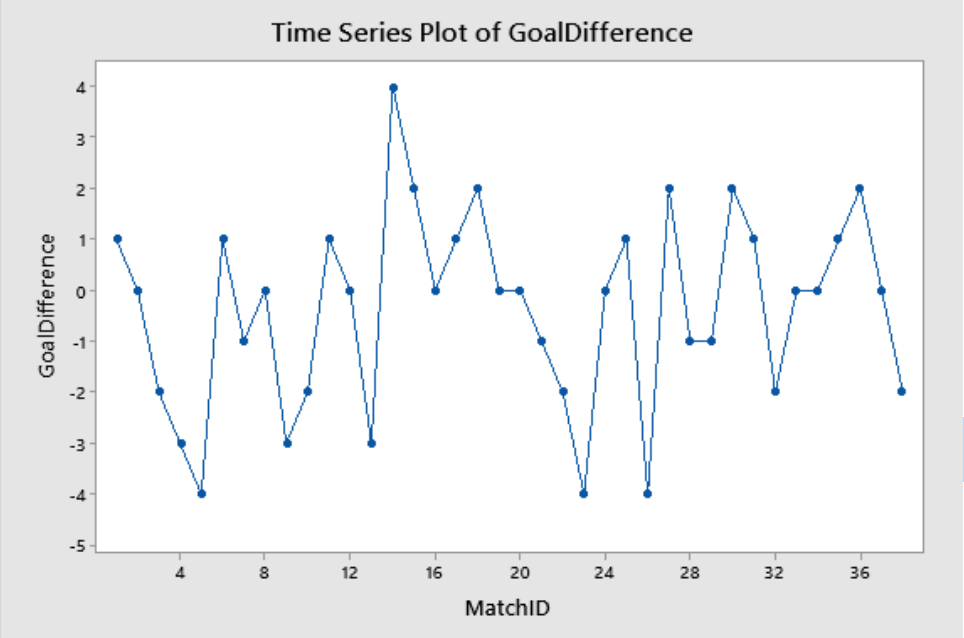
\includegraphics[scale=0.5]{images/GoalDifference.png}
\caption{Goal Difference for the entire season}
\end{center}
\end{figure}\\
Game 14 started off with the formation 4-4-2, experienced three substitutions from 4-4-2, 4-5-1, and finally ended at 4-6-0. Applying the matrix algorithm above, we generate the following matrix as a table.\\
\newline
\newline
\begin{table}
\begin{center}
\begin{tabular}{|c|c|c|c|c|c|c|c|c|c|c|c|c|c|c|}
\hline
D\backslash$O$ & D2 & D5 & D6 & D7 & F1 & F2 & G1 & M1 & M10 & M11 & M4 & M6 & M8 & M9\\
\hline
D2&0 & 6 & 8 & 0 & 0 & 13 & 3 & 5 & 0 & 0 & 1 & 2 & 0& 0\\
\hline
D5&5 & 0 & 0 & 0 & 3 & 7 & 3 & 0 & 2 & 1 & 2 & 4 & 3& 1 \\
\hline
D6&7 & 1 & 0 & 5& 5 & 3 & 5 & 5 & 0 & 1 & 1 & 2 & 1 & 0 \\
\hline
D7&0 & 0 & 4 & 0 & 6 & 4 & 2 & 4 & 0 & 1 & 5 & 0 & 4 & 0\\
\hline
F1&0 & 0 & 0 & 1 & 0 & 2 & 0 & 1 & 0 & 0 & 3 & 2 & 3 & 0\\
\hline
F2&5 & 9 & 8 & 2 & 4 &1 & 1 & 6 & 0 & 0 & 4 & 11 & 3 & 0\\
\hline
G1&2 & 1 & 0 & 0 & 8 & 0 & 0 & 0 & 0 & 0& 0&1 & 1 & 0 \\
\hline
M1&5&5&5&5&1&9&1&0&1&1&7&4 & 2 & 0\\
\hline
M10&0&1&0&0&0&0&0&0&0&1&0&1& 0& 0\\
\hline
M11 & 0 & 0 & 2 & 1 & 0 & 0 & 0 & 1 & 0 & 0 & 1 & 0 & 0 & 1\\
\hline
M4 &1&1&0 & 10 & 1&0&0&3& 0&0&1&5 & 4& 0\\
\hline
M6&2&3&0&2&5&6&0&5&0&0&1&0 & 4 & 0\\
\hline
M8&0&4&0&3&3&5&0&3&0&0&3&0 & 0 & 0\\
\hline
M9&0&1&0&0&0&0&0&0&0&0&1&0 & 0& 0\\
\hline
\end{tabular}
\caption{Match 14}
\end{center}
\end{table}
\newline
Then, we want to a column summation of Total Passing Players to evaluate the total number of active passes that were generated by this player. This would show us the number of actions that are generated by this player in the network. \\
\newline
\qquad \textbf{Column summation of total passing per players:}
\begin{equation*}
C(D,F,M)=\sum{((D,F,M)_n,(D,F,M)_n)}
\end{equation*}\\
From the row summation of total passing Network, we observe that the three substituted players (M9, M10, M11) have trivial effects on the summation of total passing, which each of them accounted for (2, 3, 6). \\
\newline
We then proceed to do a row summation of this matrix, this would give us the number of passes that are received by this player. It is important to acknowledge this fact as both ends in the passes of soccer are important.\\
\newline
\textbf{Row summation of total passing per players:}
\begin{equation*}
R(D,F,M)=\sum{((D,F,M)_n,(D,F,M)_n)}
\end{equation*}\\
\newline
\textbf{Degree Centrality of Active Passing and Passive Receiving:}\\\newline
Based on the number of passing per players, we decide to use degree centrality to evaluate the importance of a particular node(players) in this passing network. Each passing that originates from this player will be represented as an active edge connecting to the destination players. We calculate the total sum of the active edge of each node in this network to present the amount of activity that is generated by this node. Then, we calculate the amount of activity that is received by this node to evaluate the flow of activities. 
\begin{equation*}
T(G) = \sum_{i=1}^{N} R(D,F,M)\newline \qquad
	C_{(d,p)}(G) = \frac{C(D,F,M)}{T(G)}\newline \qquad
	C_{(d,r)}(G) = \frac{R(D,F,M)}{T(G)}\newline
\end{equation*}
\newline
\newline
\newline
\textbf{Graphical Representation of Match 14 Passing Network Analysis}
\newline
\begin{figure}[ht]
\begin{center}
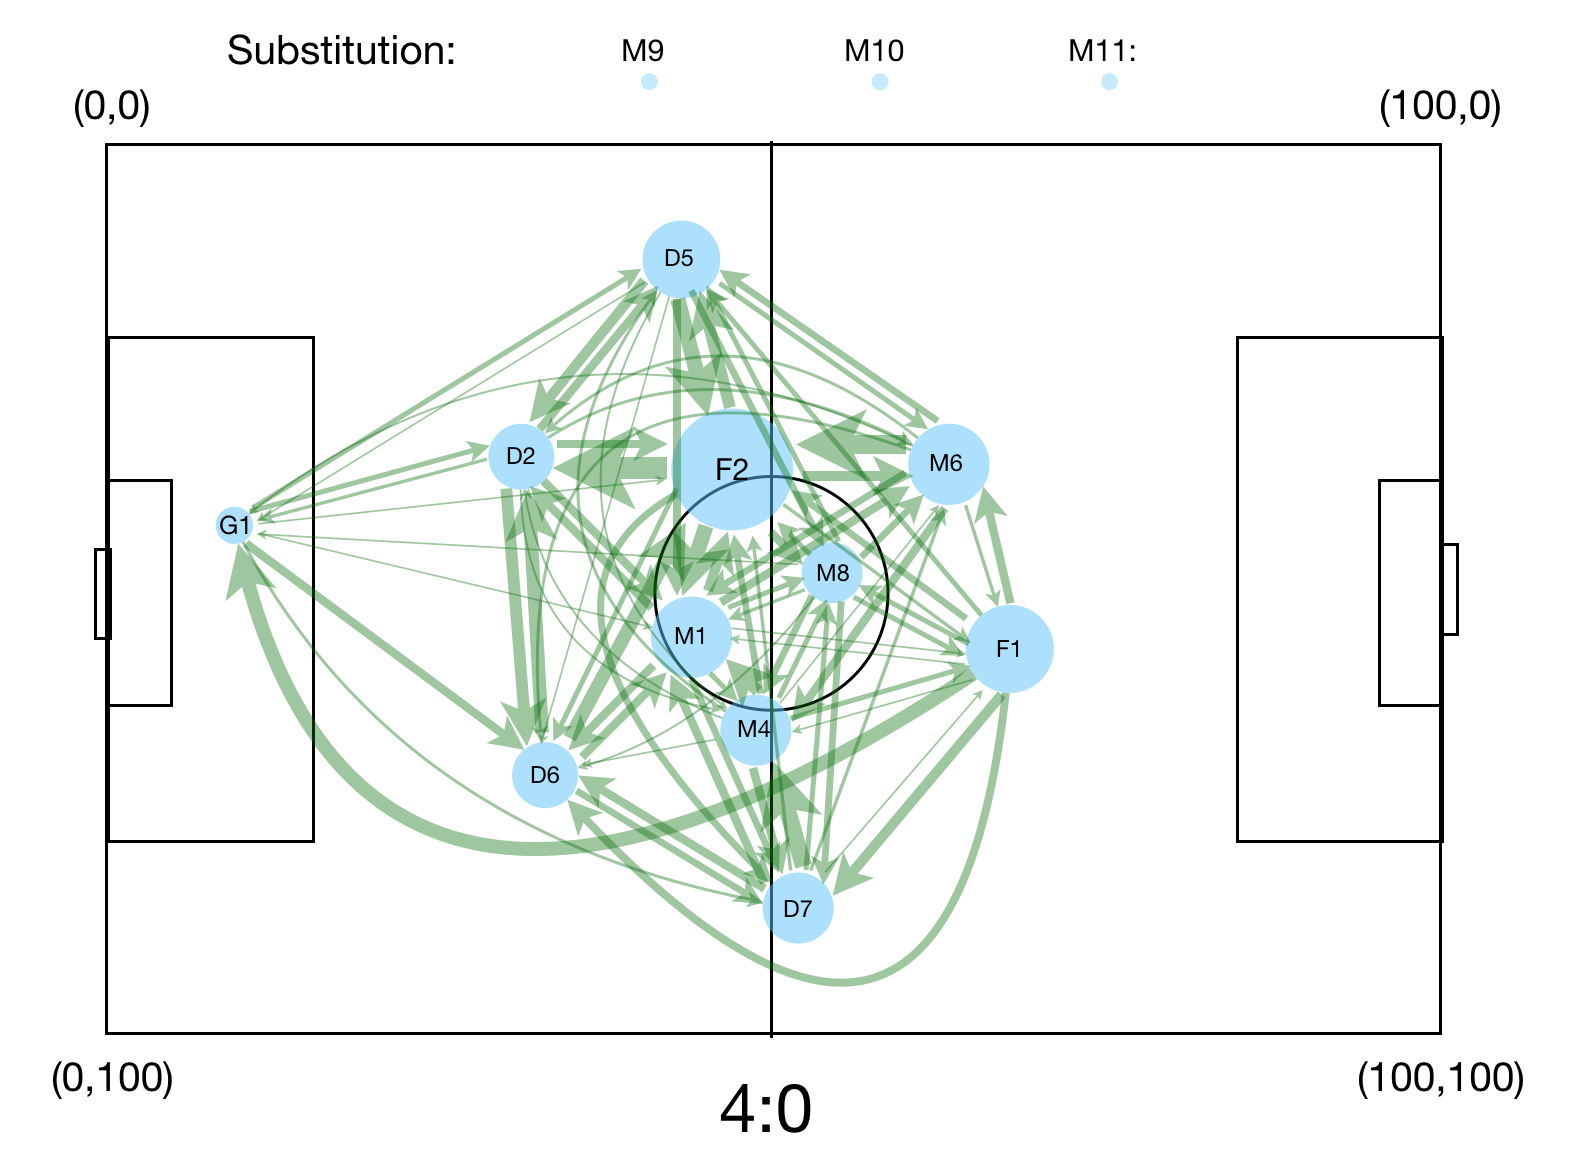
\includegraphics[scale=0.34]{images/Wingame.png}
\caption{Match 14 Passing}
\end{center}
\end{figure}\\
\newpage
\textbf{Graphical Representation of Match 23 Passing Network Analysis}
\begin{figure}[ht]
\begin{center}
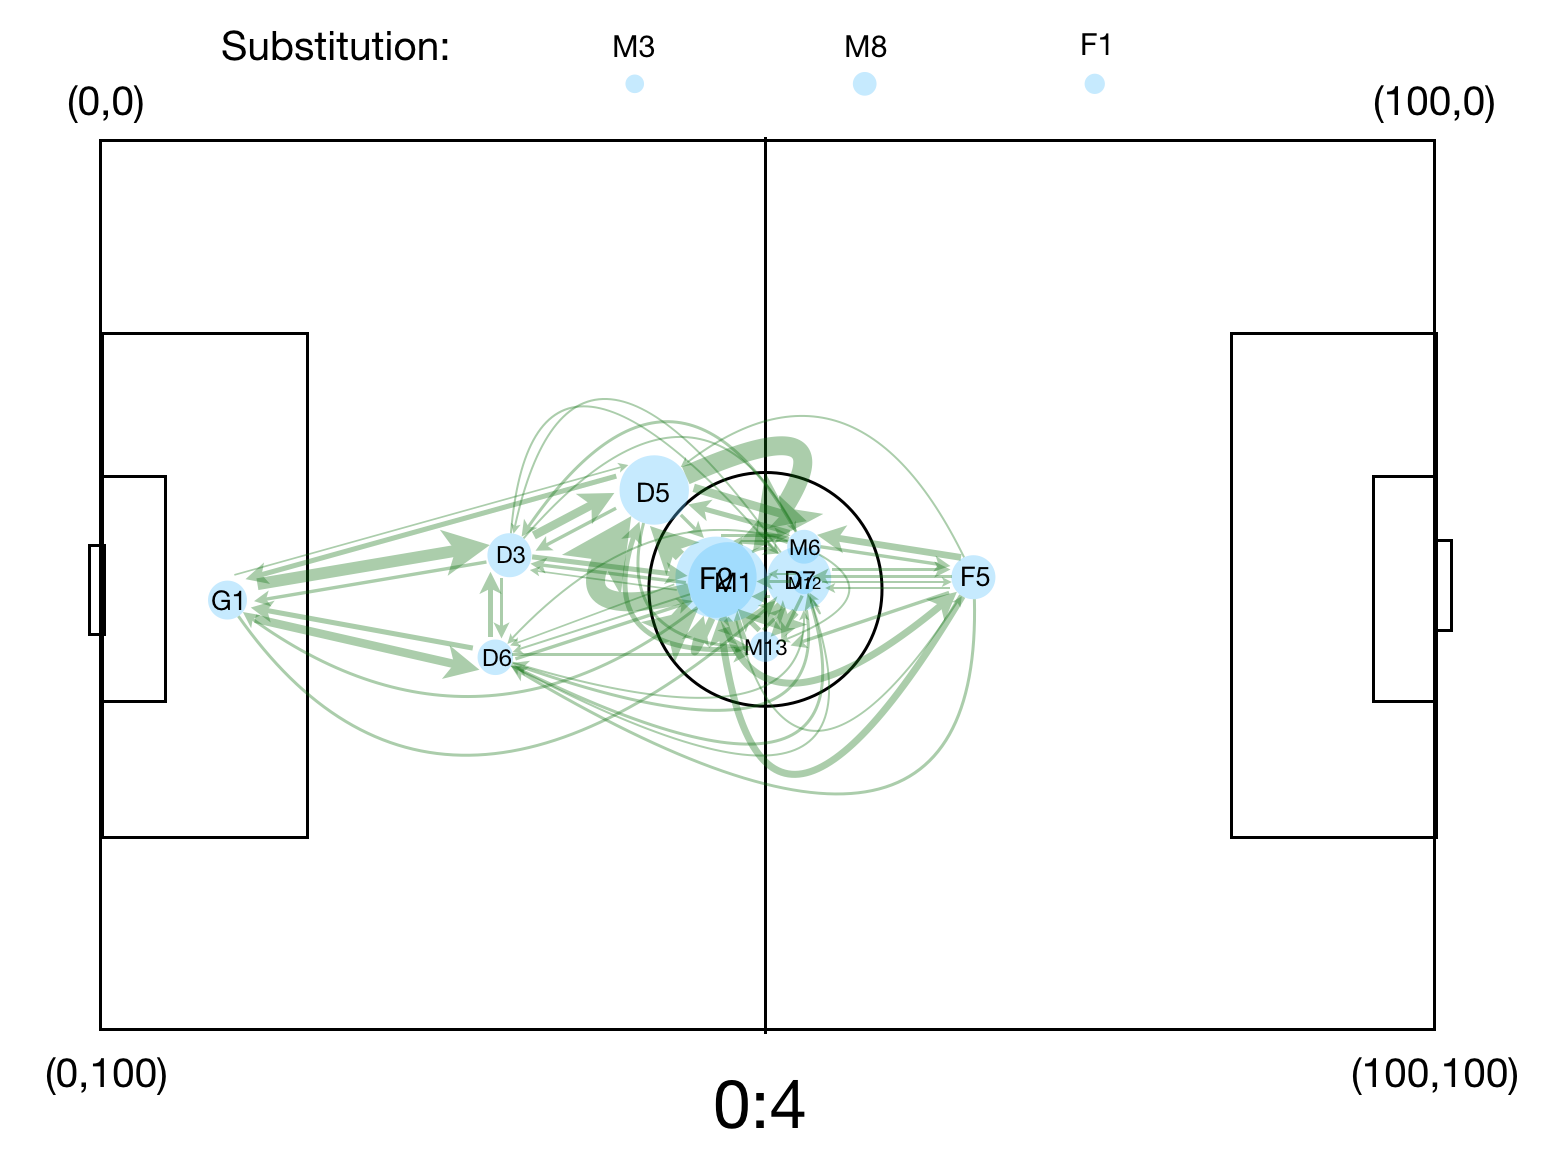
\includegraphics[scale=0.34]{images/LoseGame.png}
\caption{Match 23 Passing}
\end{center}
\end{figure}\\
From the Degree Centrality calculation of each player, we concluded that the substitution players M9, M10, M11 are relatively small in their influence, each accounted for 0.5\%, 0.8\%, and 1.7\%, to the entire Passing Network. So, we decided to put them aside and analyze the remaining 97\% percent of the network. \\
\newline
We realized that the data set of coordinates is respective to the attacking team perspective. However, since we are only concentrating on the passing network of Huskies, we set up the graph from the Huskies' standpoints, where the left-hand side of Huskies are denoted as (0,0) and the bottom right corner are denoted as (100,100). Then for each player, we put them into the players' average position throughout the match. The width of the connections is proportional to the number of connections between the two players. Lastly, the size of the node is relative to the number of passes they make. \\
\newline
From the match 14 graph, we can see that the F2 is the engine of transitioning goals from players to players as it has the largest size. In the Active Passing Degree Centrality dataset, F2 has 14.4\% of active passes in the network, ranking the first place out of 14 players. Moreover, in the Passive Receiving Data Sets, F2 also ranks to be the highest place with 15.5\%, which means that 15.5\% of the balls are transitioned through F2. And the top four players are among both datasets are Active - (F2(14.4\%), F1(10.3\%), M1(9.5\%), M6(9.5\%), Passive - (F2 (15.5\%), M1(13.2\%), D2(10.9\%), D6(10.3\%). Moreover, the entire team is spread out on both the X and Y-axis, which control the middle section of the field. This visually tells us that the Huskies have very strong control of the ball transitioning and the team is very confident in making the play.\\ \newline
However, on the contrary, match 23 Passing Network shows us a very different graph. The passing zone of the entire team is more condense as the average positions of multiple team members are squeezed in the central regions. The passes are shorter compared to Match 14 and most of the Huskies' passes are on their own half of the field. 
\begin{figure}[ht] 
\centering
    \begin{subfigure}{
        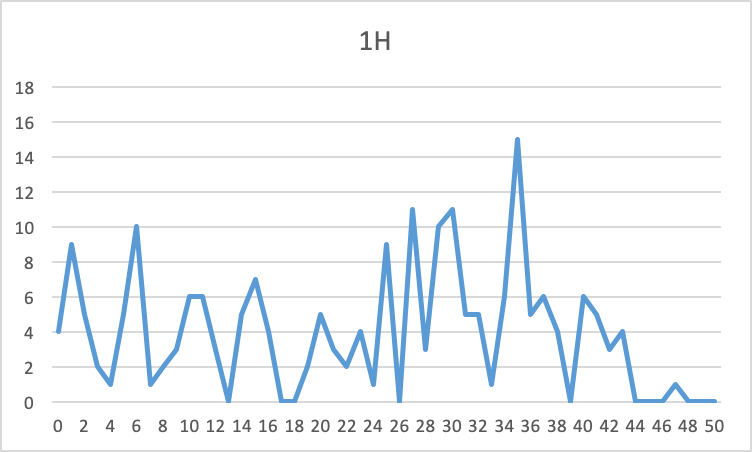
\includegraphics[width=0.38\linewidth]{images/Picture10.png}
        }
    \end{subfigure}
    \begin{subfigure}{
        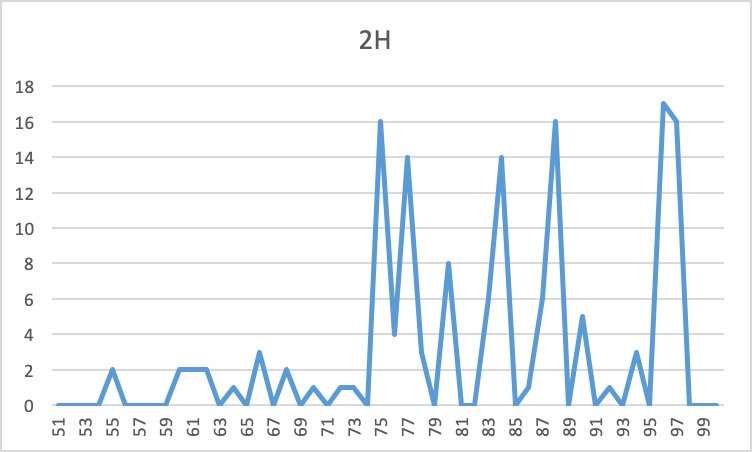
\includegraphics[width=0.38\linewidth]{images/Picture11.png}
        }
    \end{subfigure}
    \caption{Match 14: Minute to minute passing}
\end{figure}
\begin{figure}
\centering
    \begin{subfigure}{
        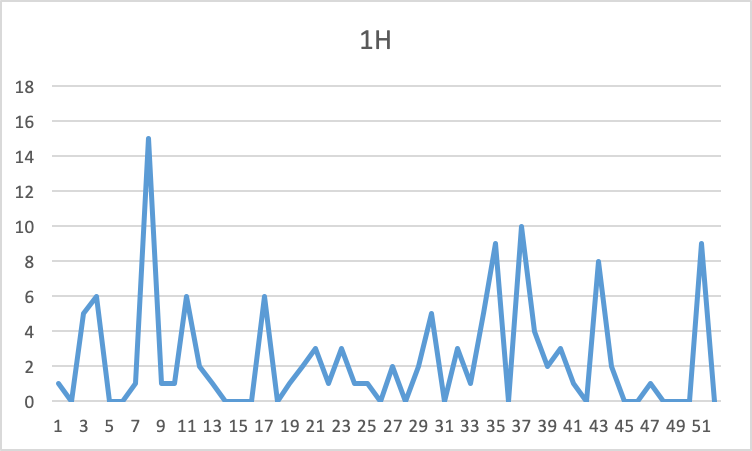
\includegraphics[width=0.38\linewidth]{images/Picture12.png}
        }
    \end{subfigure}
    \begin{subfigure}{
        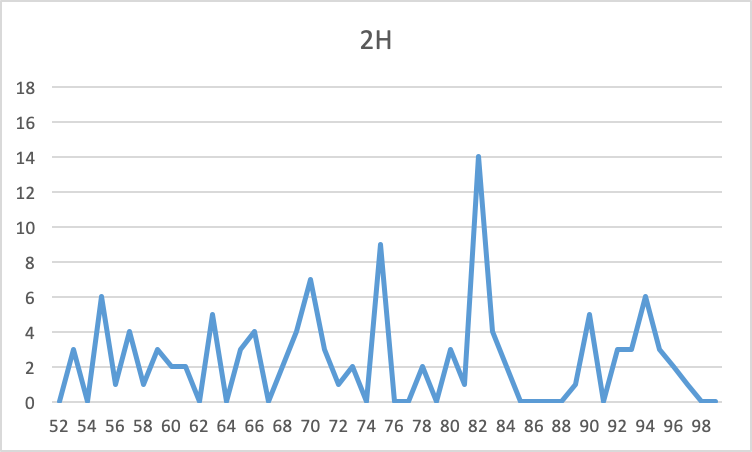
\includegraphics[width=0.38\linewidth]{images/Picture13.png}
        }
    \end{subfigure}    
    \caption{Match 23: Minute to minute passing}
    \end{figure}
\\
\newline
Moreover, the total passes throughout the game are also less than Match 14. The above graph shows the minute to minute passing between Match 14 and Match 23 with the ratio of 347 to 236  From here, we realize the correlation between effective passing and winning, and how passing can be a vital indicator of team member collaboration, winning and personal strength. 
\subsection{Passing Analysis Throughout the Entire Season}
We collect the passing events for the entire season and decide to allocate the passing events for the wins and not wins(losses and ties). Then for each dataset, we decide to average them out to see the passing pattern for this entire season. And we find a significant difference on wins and non-winning games 
\begin{figure}[ht]
\centering
    \begin{subfigure}{
        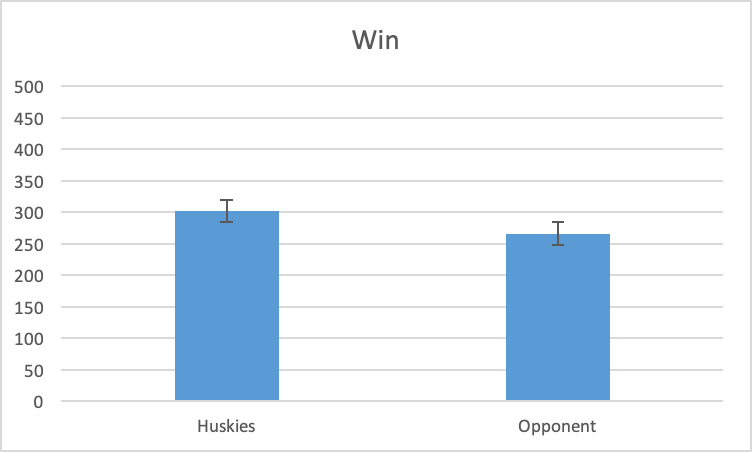
\includegraphics[width=0.38\linewidth]{images/Picture7.png}
        }
    \end{subfigure}
    \begin{subfigure}{
        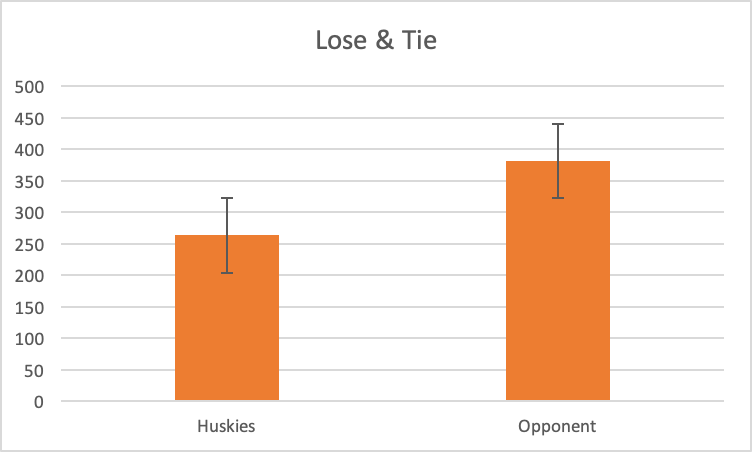
\includegraphics[width=0.38\linewidth]{images/Picture6.png}
        }
    \end{subfigure}    
    \caption{Season Passing Stats}
    \end{figure}
\\
The number of passes on the win matches outnumbers the passes on the lost matches by 50. Moreover, the number of passes for Huskies during the losing matches is significantly lower than the opponent, which usually implies a lesser control of the ball than the opponent does and less of the time which the ball is on the opponent’s field. 

\subsection{Dyadic and Triadic configurations } 

From the Graph above for Match 14, we observe that the team collaboration between each member has become a vital factor in constituting the win. For example, the interaction between F2 and M6 forms a strong pairwise connection that ensures the safety of the ball control when the attack is potentially facing a group of strong opponents that try to surround the attacking player. Moreover, the Triadic configuration between player F1, M6 and D7 helps to provide support when F1 tries to penetrate the opponent’s defense. The relationships between players help to generate more energy flow through the network. 
\newline
\begin{figure}[ht]
\centering
    \begin{subfigure}{
        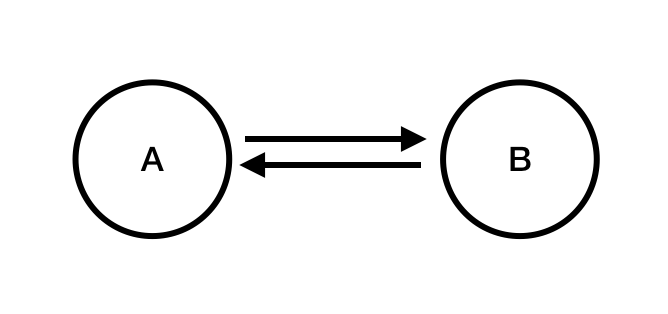
\includegraphics[width=0.2\linewidth]{images/Tri.png}
        }
    \end{subfigure}
    \begin{subfigure}{
        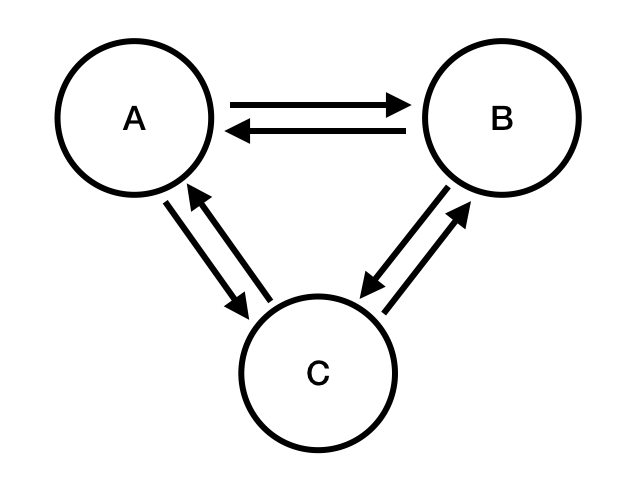
\includegraphics[width=0.2\linewidth]{images/Di.png}
        }
    \end{subfigure}    
    \caption{Dyadic and Triadic Configurations}
    \end{figure}
\newline
\begin{table}[ht]
\parbox{.5\linewidth}{
\centering
\begin{tabular}{|c|c|c|}
\hline
A & B & Frequency\\
\hline
 M1&M3&65\\
\hline
D4&M3&33\\
\hline
D5&F2&28\\
\hline
D5&M1&26\\
\hline
\end{tabular}
\caption{Dyadic}
}
\hfill
\parbox{.5\linewidth}{
\centering
\begin{tabular}{|c|c|c|c|}
\hline
A & B & C & Frequency \\
\hline
F2&M1&M3 & 10\\
\hline
D5&F2&M1 & 9\\
\hline
D1&M1&M3 & 8\\
\hline
F2 & M1 & M4 & 6\\
\hline
D6& M1 & M3 & 6\\
\hline
D2 & M1 & M3 & 6\\
\hline
\end{tabular}
\caption{Triadic}
}
\end{table}
\newline
Has formed a central structure along the middle line of the field. It represents the front base for the attacking team members to receive support and the first defense line that protects the opponent team to move further into the Huskies field. Another important configuration during Match 14 was the interaction between  F2, M1, and M4. Moreover, these two configurations overlap with F2 and M1, which further connect the entire factor. So, in order to optimize the passing network. It is vitally important to increase these interactions between players. Our advice to the coach of Huskies is that they should practice more pairwise or group of three team plays to increase the efficiency of transitioning the balls to the opponent’s field.

\subsection{Composite Degree Centrality Assessment }
From the examples and data provided above, we realize the importance of passing from multiple dimensions. If we see passing as an edge in a group, then it is important to acknowledge that both ends of the edge are equally important. Thus, we divide passing to two ends as active passing and passive receiving which both should count as an individual’s playing ability into making contributions to the entire passing network. Thus we develop the Composite Degree Centrality Model into evaluations of team members. \\
\newline
For Individual Match:  
\begin{equation*}
\frac{C_{(d,p)}(G) \times C_{(d,r)}(G)}{\sum{( C_{(d,p)}(G)\times C_{(d,r)}(G))}}
\end{equation*}
\\ For the Entire Season:
\begin{equation*}
\sum{\frac{C_{(d,p)}(G) \times C_{(d,r)}(G)}{\sum{( C_{(d,p)}(G)\times C_{(d,r)}(G))}}}
\end{equation*}\newline
Thus, we can determine the individual contribution of players into constructing the passing network. 
\newline
\newpage
\section{Danger Zone}
\subsection{Objective}
To use the \textbf{Central Limit Theorem(CLT)} to find the “Danger Zone” that reflects the most frequent region of producing shots in the future.
\subsection{Initial Model}
Since we looped over the shots produced by Huskies and collected all the possible attempts, we decided to use median ($x=88$) to show the “danger line” that is most likely to produce shots, and intuitively, any area closer to the opponent’s goal can be regarded as the “danger zone”:
\begin{figure}[ht]
\begin{center}
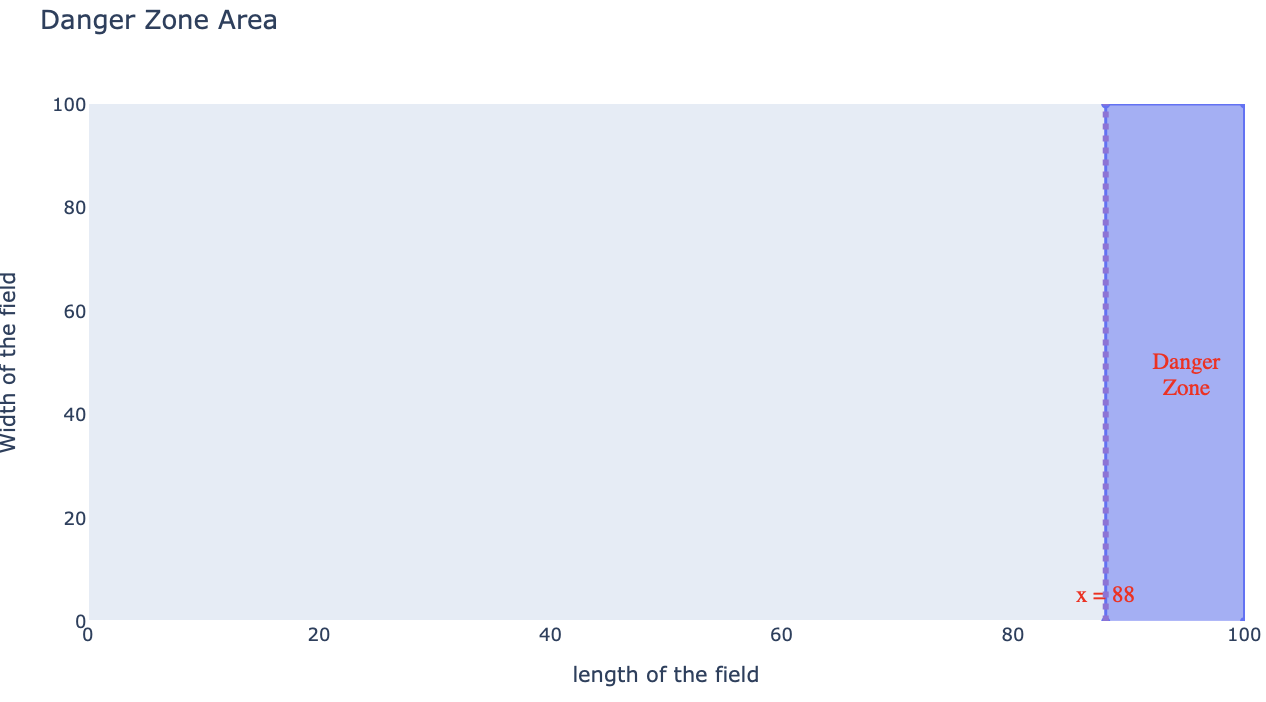
\includegraphics[scale=0.6]{images/DangerZone.png}
\caption{Danger Zone}
\end{center}
\end{figure}
\subsection{New Model}
As we observe that Figure 2 has a high standard error of $(8.989, 12.404)$ for the shot collection, we decide to use the Central Limit Theorem to find the most-likely-shot zone.
\begin{equation*}
\centering 
\mu = \frac{1}{N}\sum_{i=1}^{N} x_i  \qquad  \qquad   
\sigma = \sqrt{\frac{\sum_{i=1}^{N} (x_i-\mu)^}{N}}
\end{equation*}
\\
$\mu$ : the total mean of location of shots from winning games (the population mean)\\
$x_i$: each specific location of shots \\
$N$: total number of shots \\
$\sigma$: standard deviation of the total winning shots\\ 
By collecting all the useful shot coordinates of Huskies through last season together, we chose to pick up 119 choices as a sample size each time, which is the total number of shots Huskies made in the winning games. Then, based on the law of large numbers, we decided to do 100000 times to minimize the close heuristic effect which we want to predict the future result instead of this season. The final distribution graph we produced based on the bootstrapping result is undoubtedly similar to the normal distribution: \newline
\begin{figure}[ht] 
\centering
    \begin{subfigure}{
        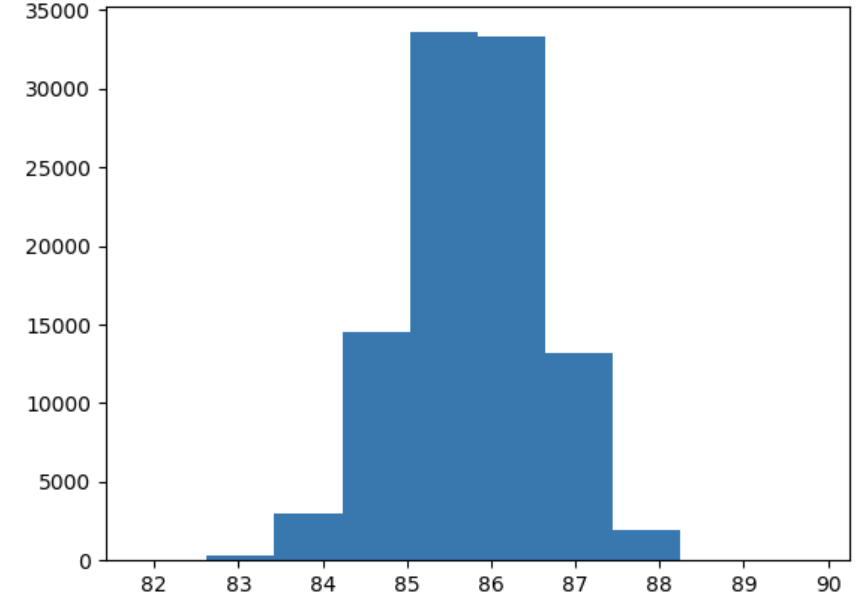
\includegraphics[width=0.45\linewidth]{images/1.png}
        }
    \end{subfigure}
        \hfill
    \begin{subfigure}{
        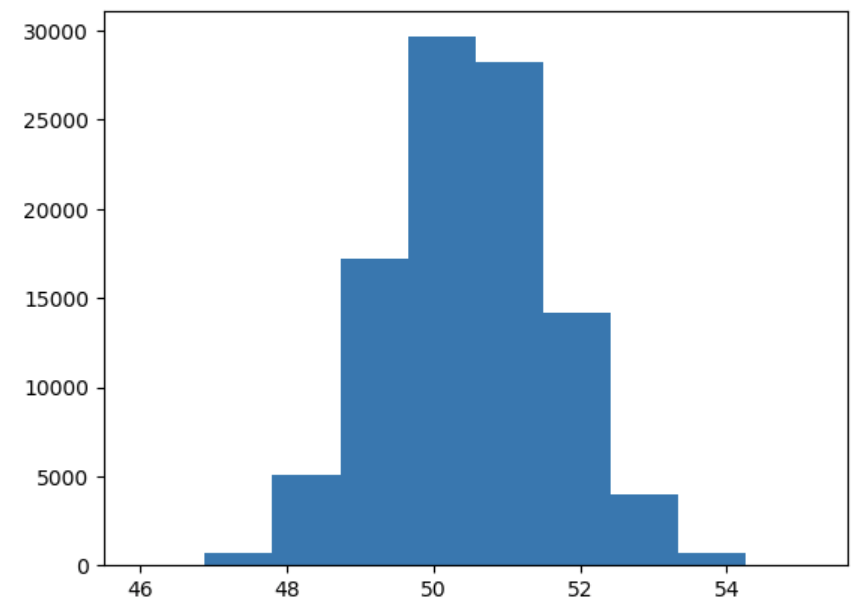
\includegraphics[width=0.45\linewidth]{images/2.png}
        }
    \end{subfigure}
    \caption{Distribution of $X$(left) and $Y$(right) coordinates}
\end{figure}
\\
As the graph shows, we can finally specify the “danger zone” as a rectangular with the coordinates: (82.62, 47.12), (82.62, 55.18), (88.27, 47.12), (88.27 55.18). Correspondingly, the standard error right now is (0.83,1.14), which is conspicuously better than the original data we extracted from this season of Huskies.\\
\begin{figure}[h]
\begin{center}
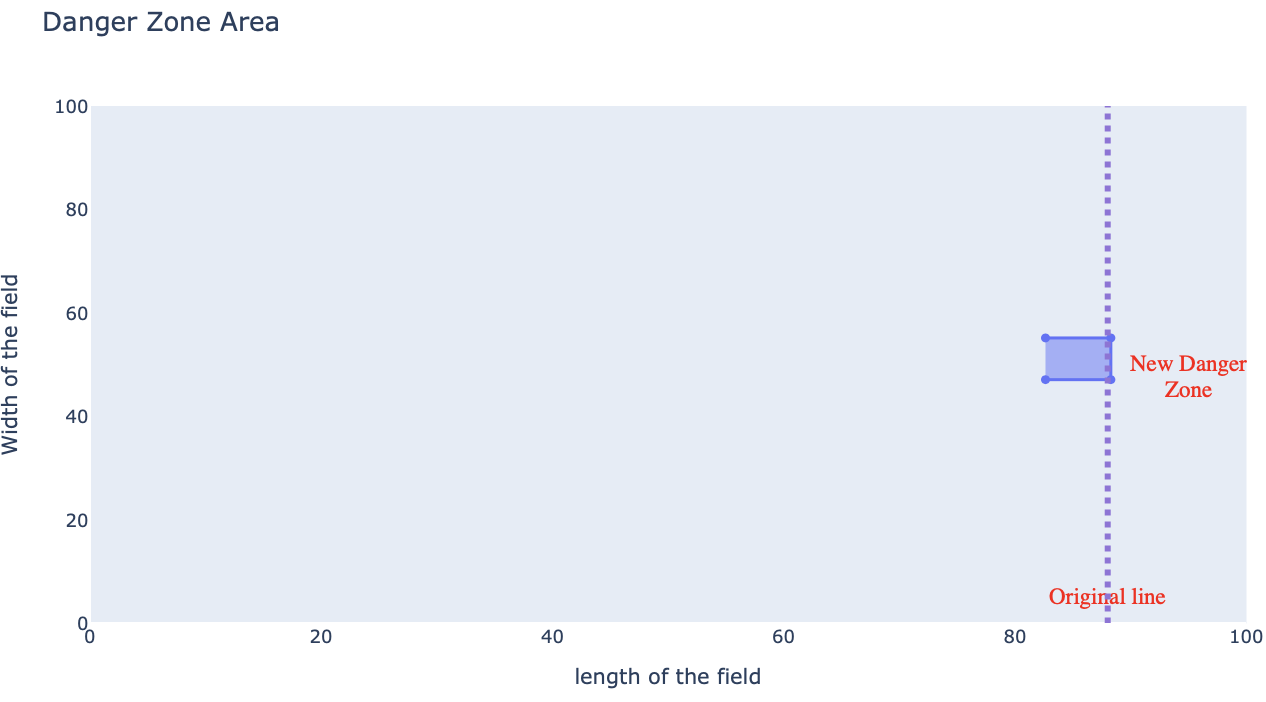
\includegraphics[scale=0.6]{images/ImprovedDangerZone.png}
\caption{Final Danger Zone}
\end{center}
\end{figure}
\newline
Now, we can say that whenever and whatever the Huskies reach out to this region, then it most likely to be counted as a successful play to produce shots. We can use this region to judge the team performance for each game and the ability of coaches to create the shooting chance for players. 
\section{Player Abilities}
\subsection{Objectives}
Through finding the best way to define the ability of any soccer player, we would like to make the following achievements: \\  1) Locating the best players among Huskies with the comparatively higher overall skills and analyze the relationship between the number of appearances of them with the winning rate and team formations. \\  2) Deciding which coaches more frequently use the best team formation with the best players in this season and which were not, then we can make the improvement around this point. \\ 3) Find the bottom ability players, so that we can adjust their positions with the team formation or even trade off.
\subsection{Team Model}
We first need to analyze which kinds of data can be used to define the ability of players from the database we have. After researching on the relevant articles, we finally came across one paper called Characteristics That Make A Good Soccer Player. It describes the ability of any soccer player as team work, intelligence, attitude and concentration. Since we only have limited data set and simple code name, we decided to use the Duel, Pass, Foul, Shot and Interruption to define the players’ skill sets. However, as we looped over the whole database, there only occurs four times interruptions, but for the other aspect we can receive a pretty decent amount of number to analyze, thus we decided to drop Interruption out of consideration. 
In order to reflect the accurate skill level from each aspect for each player, we would like to create a simple equation as: 
\begin{equation*}
 E_t= E_d + E_p + E_f + E_s
\end{equation*}
\newline
Here, we define $E_t$, $E_d$, $E_p$, $E_s$ respectively as the total efficiency for each player, the efficiency of Duel, the efficiency of Pass and the efficiency of Shout.
\\
\newline
In order to reflect the efficiency of each component from database, we think that the most efficient way to achieve the result is to use this formula:
$E(s) = \frac{N}{P} $, where x stands for the total number of $s$ and $P$ stands for the total number of game the player participated. We decide to regard the efficiency as the amount of the specific action he can make per game, by
calculating the total number of a specific aspect from the player ($N$) and divide it with the number of played games ($P$), since each player had played different times last season as shown below: 
\newline
\newline
\newline
\begin{figure}[h]
\begin{center}
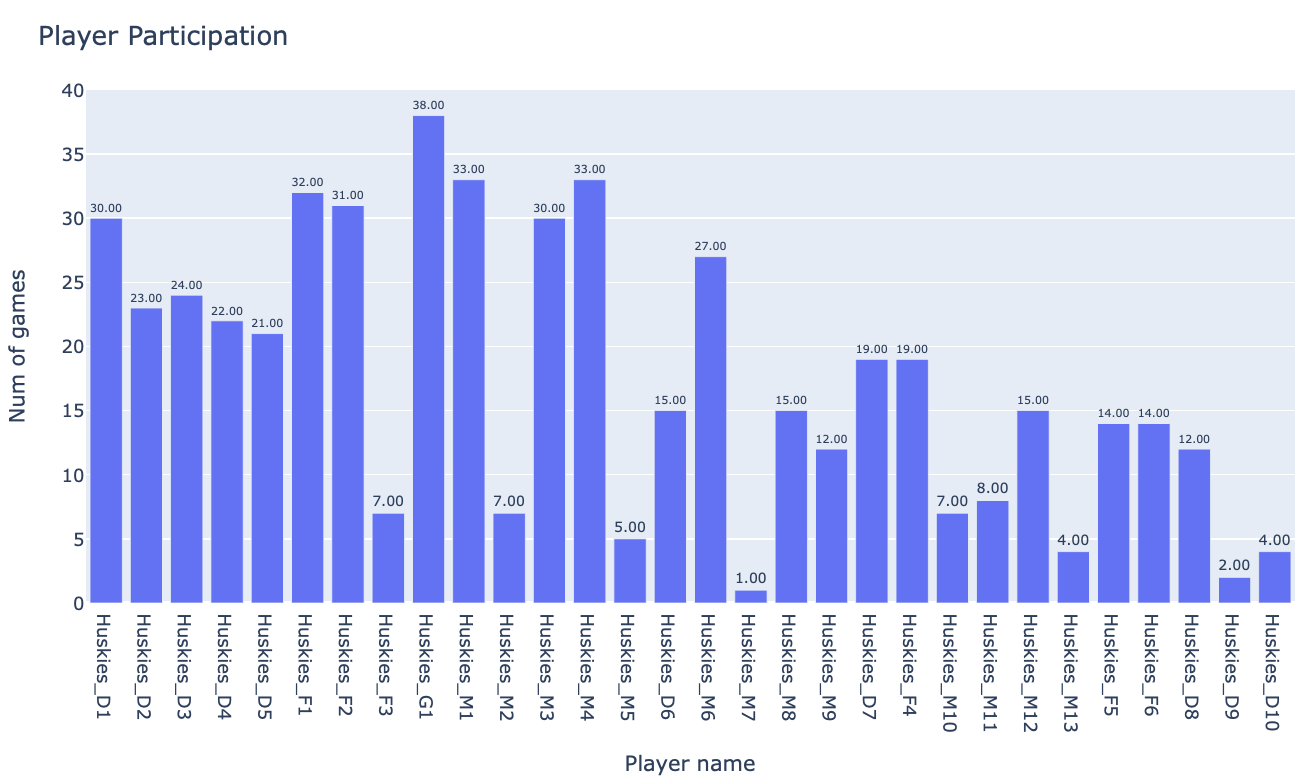
\includegraphics[scale=0.5]{images/3.png}
\caption{Player Participation}
\end{center}
\end{figure}
\newline
\newline
Then following the calculation,we encounter this problem of raw data unbalancing as they have different parameters.\newline
\begin{figure}[h]
\begin{center}
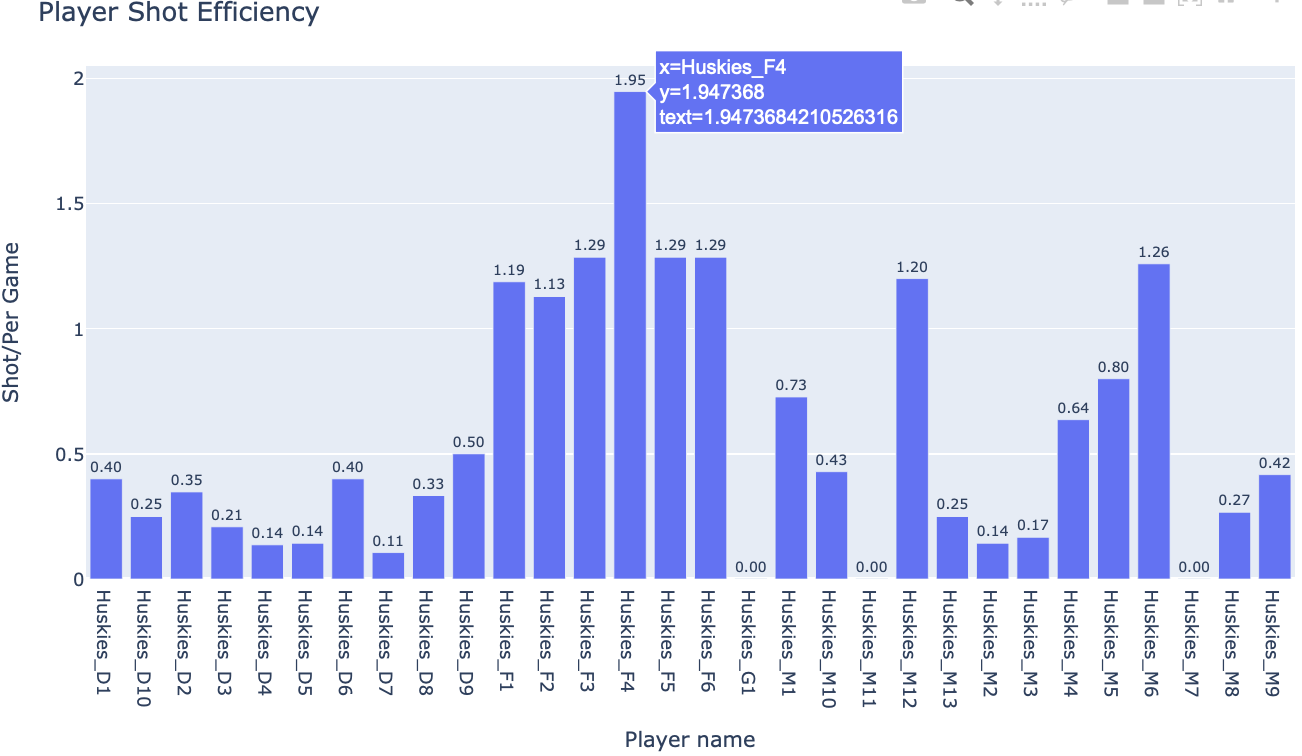
\includegraphics[scale=0.5]{images/4.png}
\caption{Player Shot Efficiency}
\end{center}
\end{figure}
\begin{figure}[h]
\begin{center}
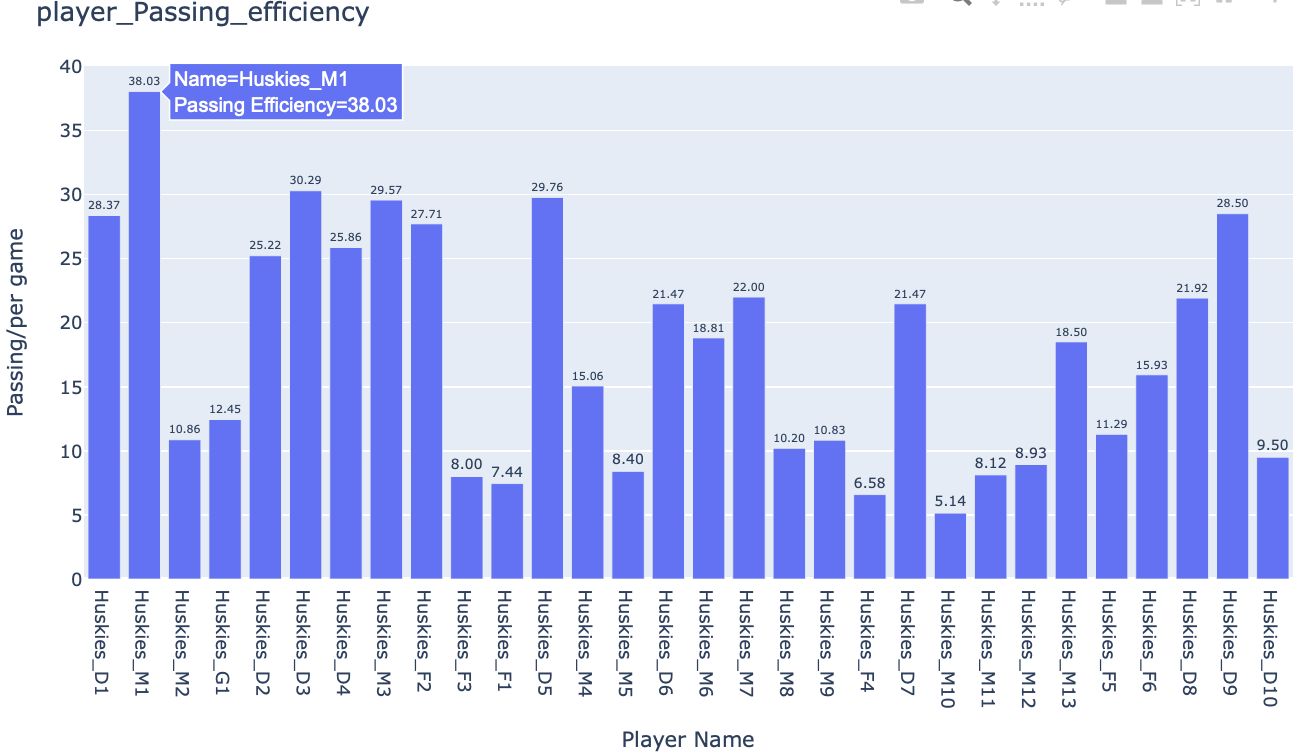
\includegraphics[scale=0.5]{images/5.png}
\caption{Player Passing Efficiency}
\end{center}
\end{figure}\newline
\newline
\newline
\newline
\newline
\newline
\newline
\newline
As the graphs show, the efficiency of passing is much higher than the efficiencies of Shot, and indeed Duel and Passing are much higher than the rest, so we can not directly use the raw score, thus instead, we create this curving function: 
\begin{equation*}
    f(x) = \frac{100x}{H}
\end{equation*}
(Function represents that the highest one ($H$) in each aspect will become 100\% and the other ones are computed as the percentage of H they attained) 
By applying the formula, the data becomes more representative as:
\begin{figure}[h]
\begin{center}
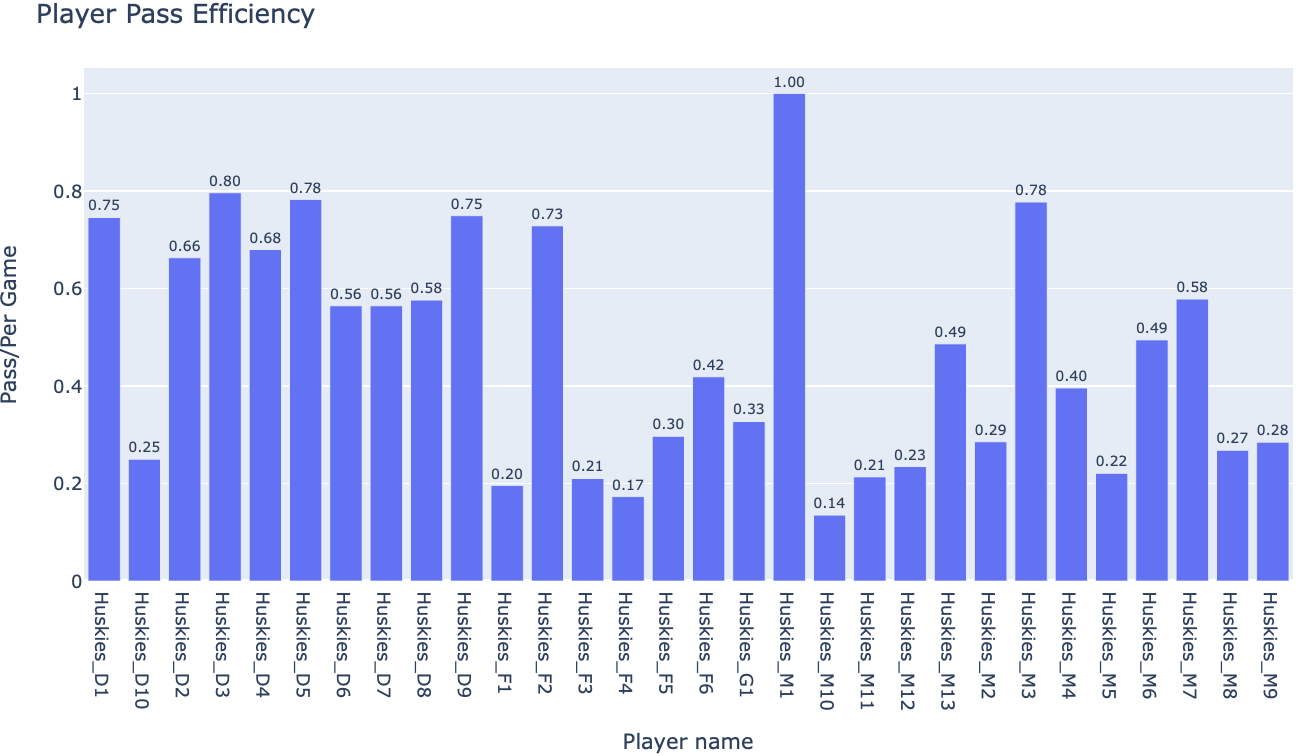
\includegraphics[scale=0.5]{images/6.png}
\caption{Player Pass Efficiency}
\end{center}
\end{figure}\newline
We approach the same method for Foul Efficiency, Duel Efficiency and Shot Efficiency (see in Appendix).\newline
Also, since we calculate the foul efficiency as how many fouls a player can produce per game, so should be counted as a negative factor. Therefore, the new equation should be: 
\begin{equation*}
 E_t= E_d + E_p - E_f + E_s
\end{equation*}
Thus, we can right now locate the best players and worst players for each position since we have their specific efficiency percentage of different divisions. 
\subsection{Division Model}
After reranking all the players, we find these following results:\\
\newline
*We assume that Goalkeeper should not be ranked since there is no substitution and intuitively he can not make many contributions on these aspects. \\
\newline
\begin{table}[ht]
\begin{center}
\begin{tabular}{|c|c|c|c|c|c|}
\hline
Type\backslash $Ranking$ & Top1 & Top2 & Top3 & Top4 & Worst1\\
\hline
Forward & 1.66 F6 & 1.20 F2 & 1.12 F3 & 1.10 F4& 0.81 F5\\
\hline
Midfielder & 1.44 M6 & 1.33 M1 & 1.08 M12 & 1.00 M7 & 0.31 M10\\
\hline
Defender & 1.29 D1 & 1.26 D3 & 1.23 D8 & 1.17 D9 & 0.21 D10\\
\hline
\end{tabular}
\caption{Total Efficiency}
\end{center}
\end{table}
\newline
From the table above, we can see that F6, M6, and M1 are the most valuable players from all dimensions. However, to make the ranking fairer for each position, we decide to rank again with the specific traits that are more relevant to them. For example, forwards should be hinged on the Shot and Duel Efficiency, defenders and the midfielders should be analyzed from Pass, Duel, and Foul Efficiency. 
\begin{equation*}
 E_t= E_d + E_s
\end{equation*}
\begin{table}[ht]
\begin{center}
\begin{tabular}{|c|c|c|c|c|c|c|}
\hline
Type\backslash $Ranking$ & Top1 & Top2 & Top3 & Top4 & Top5 & Worst1\\
\hline
Forward & 1.82 F4 & 1.61 F1 & 1.52 F5 & 1.44 F6& 1.14 F2 & 0.99 F3\\
\hline
\end{tabular}
\caption{Forward}
\end{center}
\end{table}\newline
However, from the \textbf{former Passing Network}, we find that F2 is more inclined to pass so we can not simply judge him based on this standard. Yet, F3 is relatively below others’ ability.\newline 
\begin{equation*}
 E_t= E_d + E_p - E_f
\end{equation*}\newline
The ranking is:\newline
\begin{table}[ht]
\begin{center}
\begin{tabular}{|c|c|c|c|c|c|c|c|c|c|}
\hline
Type\backslash $Ranking$ & Top1 & Top2 & Top3 & Top4 & Top5 & ... & Worst1 & Worst2\\
\hline
Midfielder & 1.01 M7 & 0.96 M1 & 0.80 M6 & 0.67 M9 & 0.63 M3 &... & 0.12 M2 & 0.09 M10\\
\hline
\end{tabular}
\caption{Midfielder}
\end{center}
\end{table}
\newline
We can now put M7, M1, M6 into the final top Midfielder list, and vice versa for M10, M2. 
\newline 
\begin{equation*}
 E_t= E_d + E_p - E_f
\end{equation*}\newline
The ranking is:\newline
\begin{table}[ht]
\begin{center}
\begin{tabular}{|c|c|c|c|c|c|c|c|c|c|}
\hline
Type\backslash $Ranking$ & Top1 & Top2 & Top3 & Top4 & Top5 & ... & Worst1 & Worst2\\
\hline
Defender & 1.16 D3 & 1.08 D1 & 1.06 D8 & 0.92 D9 & 0.89 D4 &... & 0.62 D2 & 0.08 D10\\
\hline
\end{tabular}
\caption{Defender}
\end{center}
\end{table}\newline
From the ranking above, D3, D1, D8 are ranked into the final top Defender list and add D2, D10 into the worst list. \\
\newline
So far, the top player list we have are: F4, F1, F5,  F2, M7, M1, M6, D3, D1, D8; and the worst player are: F3, M2, M10, D2, D10.To double-check their team collaboration with the whole team, we decide to combine with the team configurations.\\
\newline
According to Table 2 and 3, we can conclude that M1, D3, D1 are the most important core players for Huskies since plays almost all include him, but M3 has a high chance to cause the foul and lower chance of duel so his ability score is not conspicuous from the rankings. \\
\newline
By locating all the games that the top players were included, we find F2 played all the 10 winning games and no matter which coach could lead the team, they won nonetheless, so we can conclude that F2 should also be in the core list. However, for M1, D3, D1, among the games they all attended, they won 6 times, tied 7 times and only lost 5 times, which occupies 34\% of the winning rate, there seems to be no difference, so we can conclude those core players are not the significant determinator for winning. However, for D3, all the games he has not played, the Huskies only won 3 times. For the worst players, M2 has the highest amount of lost games (6), and then F3, M10, and D10, but the game D2 played has the highest amount of winning games (9), so we can then delete him from the worst player list. \\
\newline
Then from all the analyses, we can now decide the players to be traded in the future: M2, F3, M10; and F2 D3 are the player most important for the team. \\
\newline
By combining the frequency of team formation with the core player in the games, we find that under 4-2-2 and 4-3-3 formations, they can maximize the ability of core players and they won most times. Therefore, in the future, this can be counted as criteria to follow if we can reasonably assume core players will not leave the team. Also, even though coach 3 led most of the games in the past season, and there is a high probability that coach 1and coach 2 will use different strategy, but so far, we can see from the table,  coach 2 did not use the most winning formation frequently and the only two he coached are all with the formation as 4-2-2. Therefore, we can make the conclusion that coach 2 may need to try more winning formation (4-2-2,4-3-3) in the future if possible. Here is a graph shown the formation frequency of Coach 2:\\
\begin{figure}[h]
\begin{center}
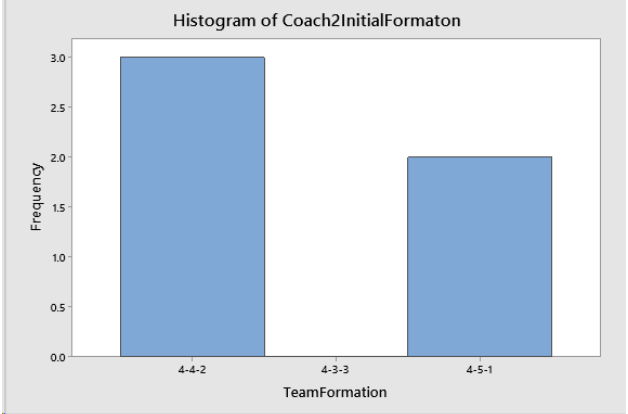
\includegraphics[scale=0.5]{images/coah.png}
\caption{Coach2 Stats}
\end{center}
\end{figure}
\section{Further Discussion}\\
\newline
\begin{figure}[h]
\begin{center}
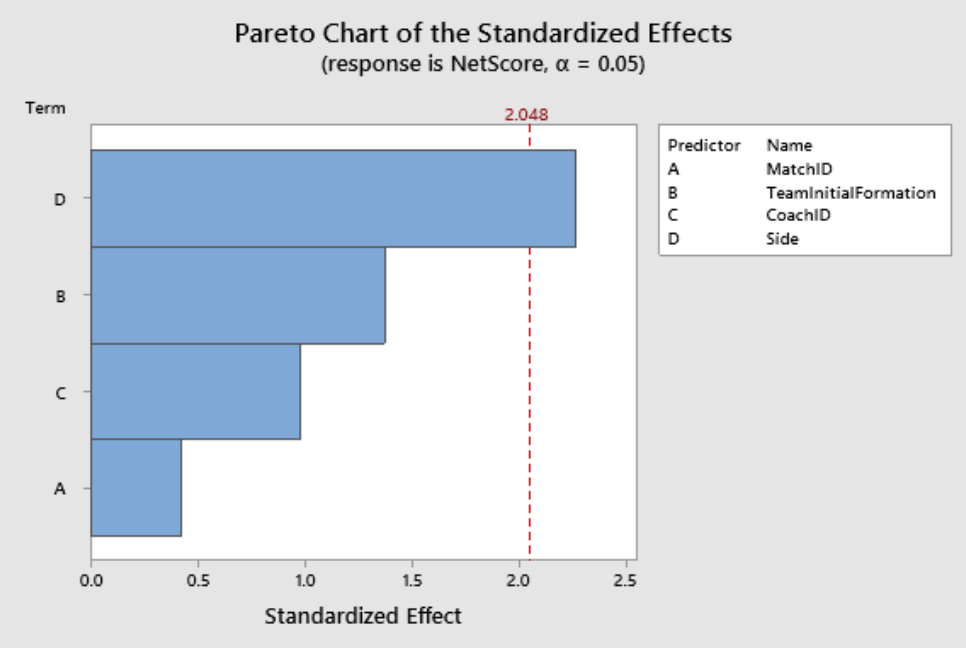
\includegraphics[scale=0.6]{images/fur.png}
\caption{Regression of outcomes}
\end{center}
\end{figure}\\
\newline
Since after analyzing the relationship between winning games and the other aspects (formation, coach, side), we find that coaches do not have a dominant influence on the outcomes of games, so besides the advice of changing formation, it is not necessary to make further discussion at this moment. However, whether playing at home or away is the biggest determinator among all the aspects, but the schedule normally can not arrange by the team itself, so we do not have the ability to make improvements in this aspect. 
\newpage
\section{Evaluation}
\subsection{Strength}
Before creating each model, we carefully cleared the data set to efficiently minimize the noises and outliers from the miscellaneous data, then we save plenty of time on finding the useful information. \\
\newline
Our models are multi-dimensional. Our models not only represent the different layers from the shallow to the bottom to prove our final thesis, but we also analyze the data from different perspectives, such as the Player Efficiency and Coach Formation Frequency and so on. Therefore, we can depict a comprehensive picture consisting of various aspects. \\
\newline
Last but not least, the models we have can be kept for future use. Since “danger zone” and the diagrams of different types of configurations can all reflect the team’s characteristic; and this team trait normally is consistent for several seasons, then the Huskies can make a constructional plan based on the drawbacks we analyze from the features. 
\subsection{Weakness}
There exist flux and unpredictable differences between our models and the real-world situation. Since from the databases we can analyze, they are not included the scoring time and the corresponding player, so we cannot take the efficiency of shot and cut-in for specific players into consideration, and we cannot make a precise conclusion about the efficiency of attacking for each game. Then, when we evaluate the attribute of each player, we lack enough information. \\
\newline
Some information is arbitrary. As for the coaches most frequent formations, we cannot directly find the formation coach used to produce a positive effect, since there is no scoring time for both sides and there is no information of weathers, so we cannot confidently say that certain type of team formation can make a great contribution for different coaches. Therefore, we can only evaluate the starting team formation for each coach, and make a consequent analysis. 
\subsection{Future Improvement}
First, with more available time, we can enhance our description of the “danger zone”. If we can convert the cartesian coordinates into real field size, then we can give a more visual-friendly diagram to reflect the real world condition. Also, we can further discuss which certain types of plays (strategies) can attain the scoring zone more easily. \\
\newline
Second, we assume no injury for all players throughout the season, but if we can then analyze the dynamic changes of each player’s statistics, the assumption is possible to become a data-supported fact. Also, we only try a little on this part because of the limitation of time, such as:
\begin{figure}[ht]
\begin{center}
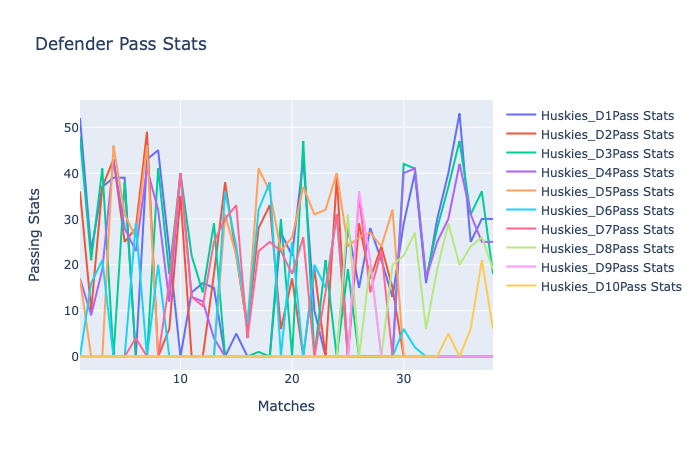
\includegraphics[scale=0.5]{images/D.png}
\caption{Defender Pass Stats}
\end{center}
\end{figure}
\\
\newpage
Third, we can make each graph more precisely. As for the graph of coaches’ formation frequency and passing dynamical pattern, sometimes we do not have the legend to decorate the graph, so they are not informative if we do not make additional explanations. 

\newpage
\begin{thebibliography}{}
 
      
 \bibitem{Av}
     Alto, Valentina. “Visualizing the Central Limit Theorem with Python.”  \emph{Medium}, Towards Data Science, 1 Aug. 2019, towardsdatascience.com/visualizing-the-central-limit-theorem-with-python-e89d2ce41788.
      
 \bibitem{Ch}
      “Characteristics That Make A Good Soccer Player.” \emph{Puget Sounds Slammers}, 28 Nov. 2017, pugetsoundslammers.org/characteristics-that-make-a-good-soccer-player/. 
      
\bibitem{CC}
     Claywell, Charlie R. “What Is Social Network Theory?” \emph{LoveToKnow}, LoveToKnow Corp, socialnetworking.lovetoknow.com/What-is-Social-Network-Theory.
\bibitem{GJ}
      Golbeck, Jennifer. “Analyzing Networks.” \emph{Introduction to Social Media Investigation}, Syngress, 20 Mar. 2015, www.sciencedirect.com/science/article/pii/B9780128016565000214.
      
\bibitem{RD}
      Richeson, Dave. “How to Curve an Exam and Assign Grades.”  \emph{David Richeson: Division by Zero}, 23 Mar. 2011, divisbyzero.com/2008/12/22/how-to-curve-an-exam-and-assign-grades/.
      
     

\end{thebibliography}
\newpage

\section{Appendix}
\begin{figure}[ht]
\begin{center}
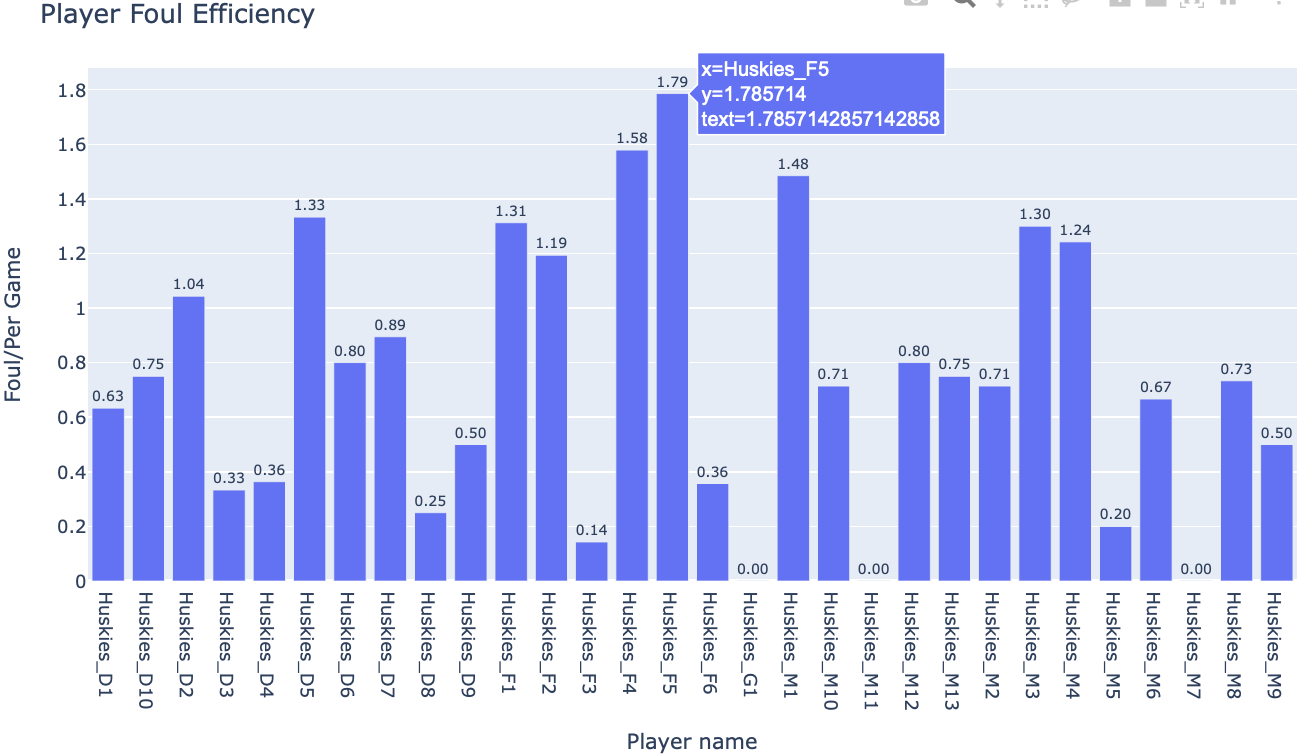
\includegraphics[scale=0.5]{images/a.png}
\caption{Player Foul Efficiency}
\end{center}
\end{figure}
\begin{figure}[ht]
\begin{center}
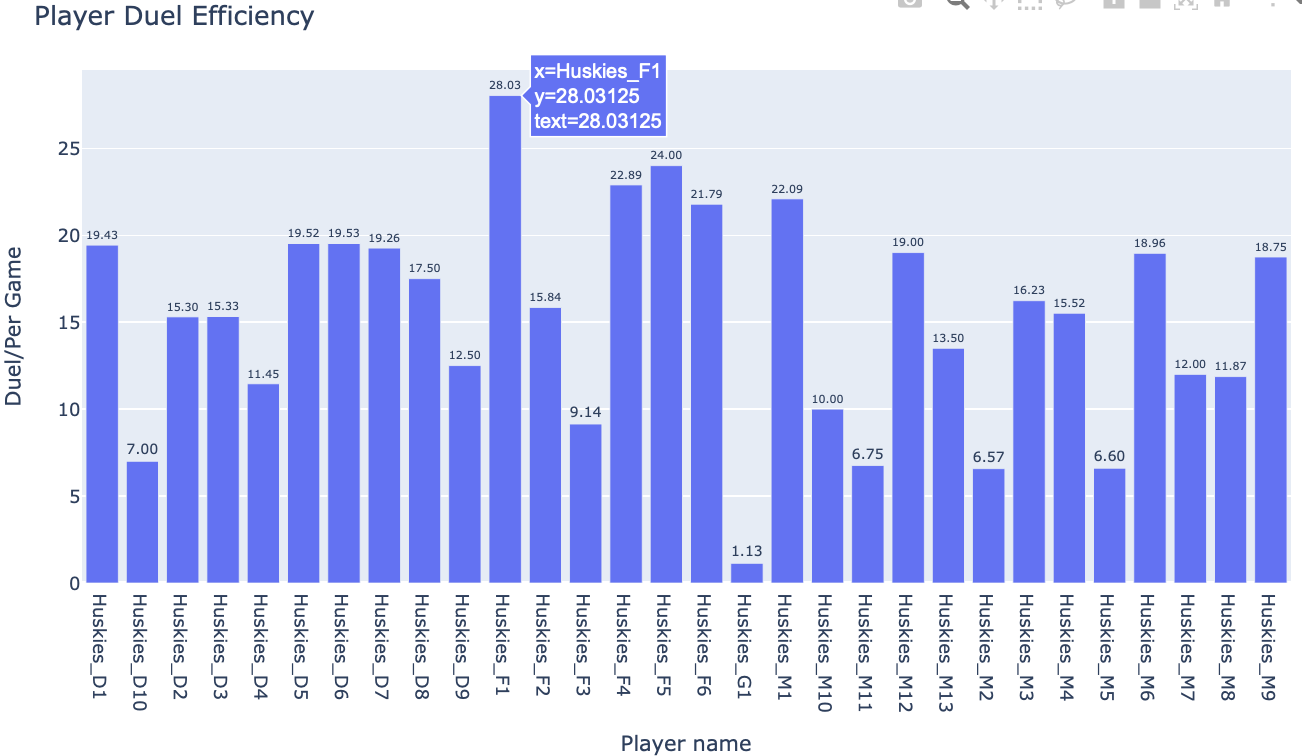
\includegraphics[scale=0.5]{images/b.png}
\caption{Player Duel Efficiency}
\end{center}
\end{figure}
\begin{figure}[ht]
\begin{center}
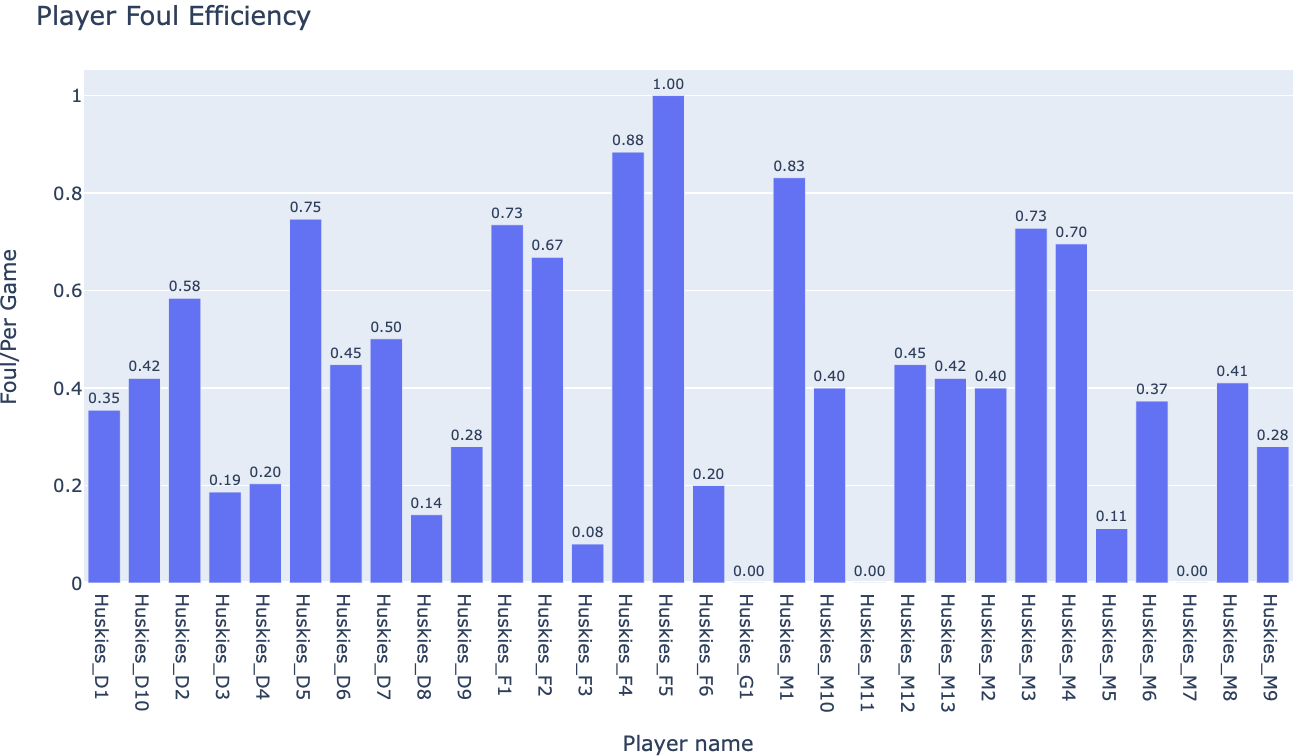
\includegraphics[scale=0.5]{images/c.png}
\caption{Play Foul Efficiency}
\end{center}
\end{figure}
\begin{figure}[ht]
\begin{center}
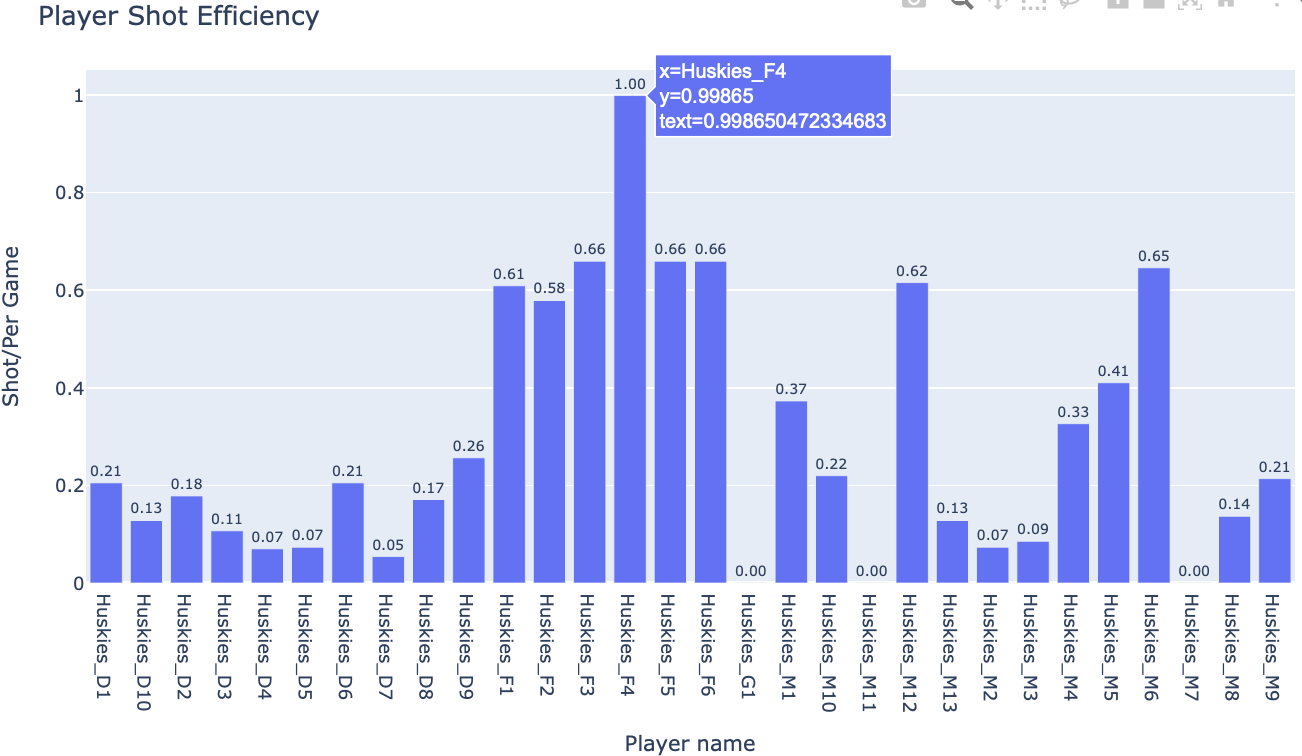
\includegraphics[scale=0.5]{images/d.png}
\caption{Player Shot Efficiency}
\end{center}
\end{figure}
\begin{figure}[ht]
\begin{center}
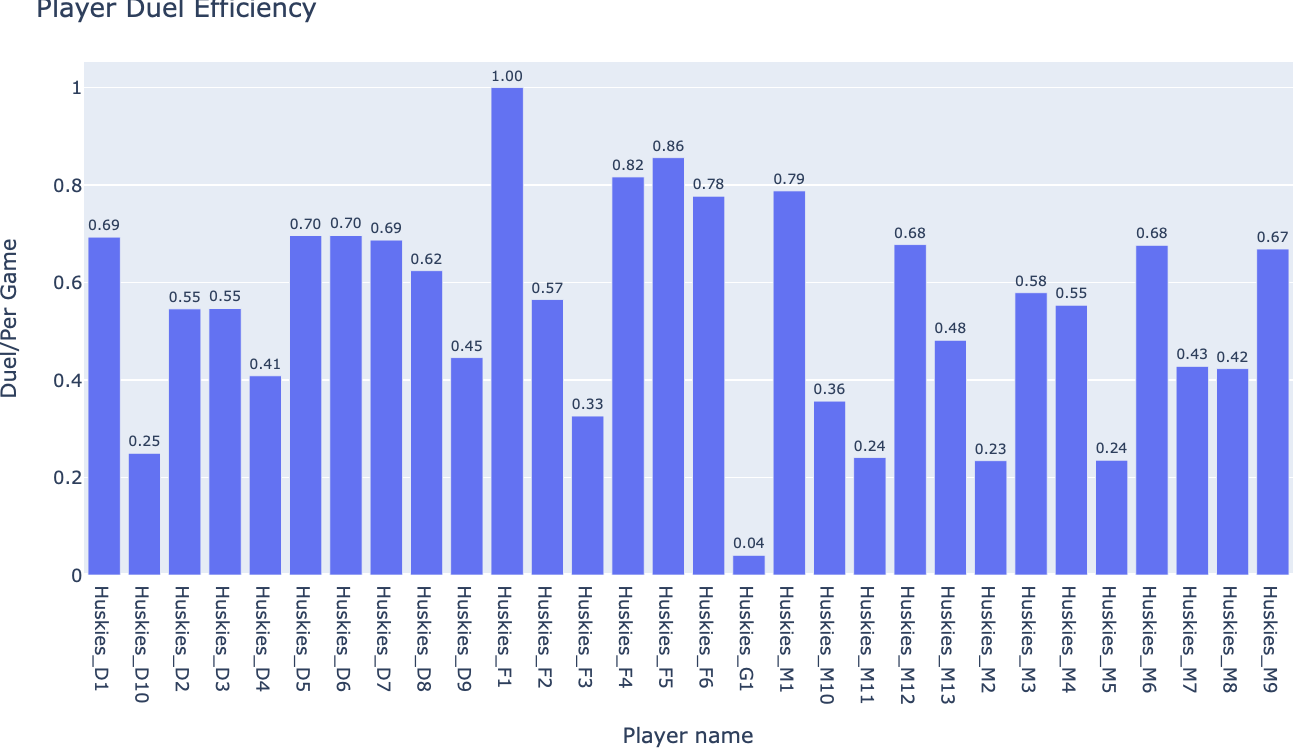
\includegraphics[scale=0.5]{images/e.png}
\caption{Player Doul Efficiency}
\end{center}
\end{figure}
\begin{figure}[ht]
\begin{center}
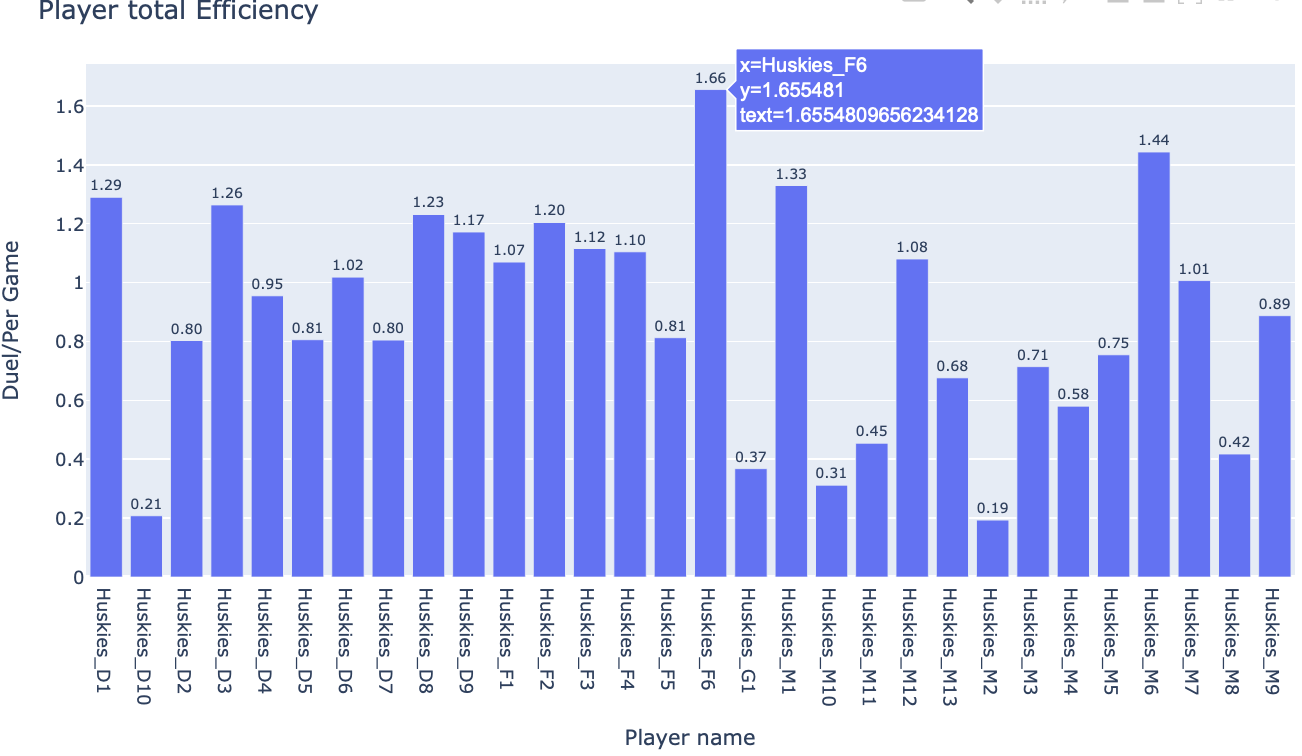
\includegraphics[scale=0.5]{images/f.png}
\caption{Player Total Efficiency}
\end{center}
\end{figure}
\begin{figure}[ht]
\begin{center}
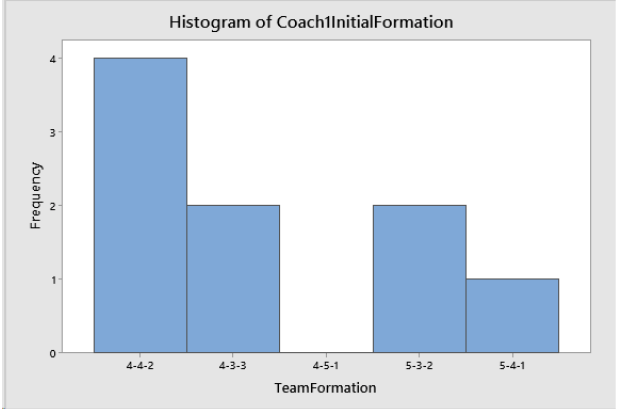
\includegraphics[scale=0.5]{images/Screen Shot 2020-02-17 at 8.29.06 PM.png}
\caption{Coach1 Initial Formation}
\end{center}
\end{figure}
\begin{figure}[ht]
\begin{center}
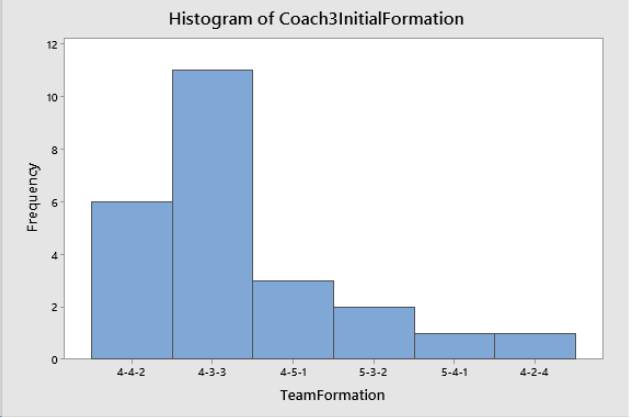
\includegraphics[scale=0.5]{images/Screen Shot 2020-02-17 at 8.29.11 PM.png}
\caption{Coach3 Initial Formation}
\end{center}
\end{figure}

\begin{figure}[ht]
\begin{center}
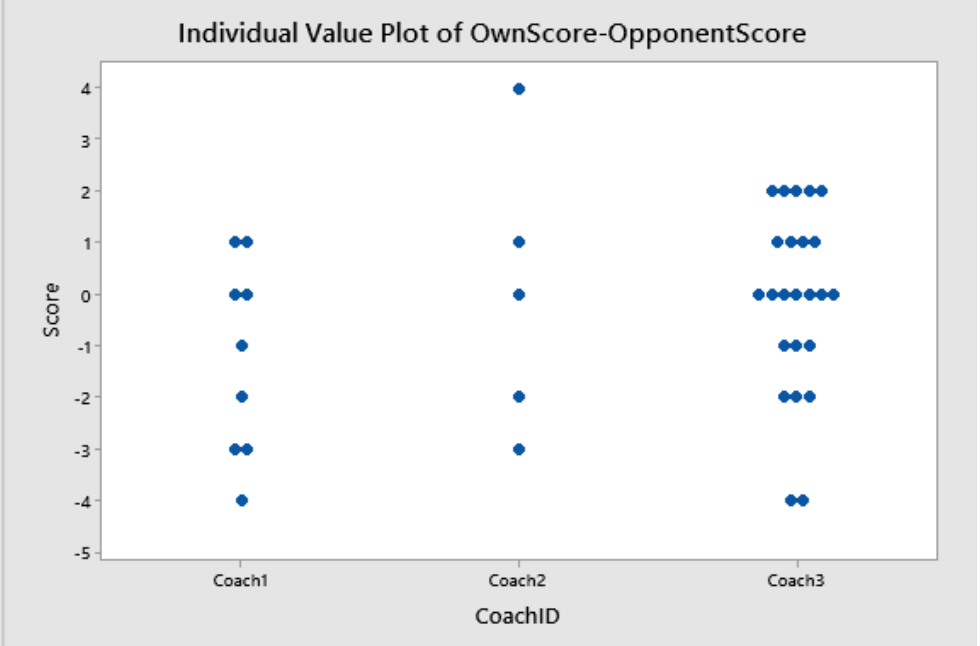
\includegraphics[scale=0.5]{images/Screen Shot 2020-02-17 at 8.29.23 PM.png}
\caption{Coach Outcomes}
\end{center}
\end{figure}
\begin{figure}[ht]
\begin{center}
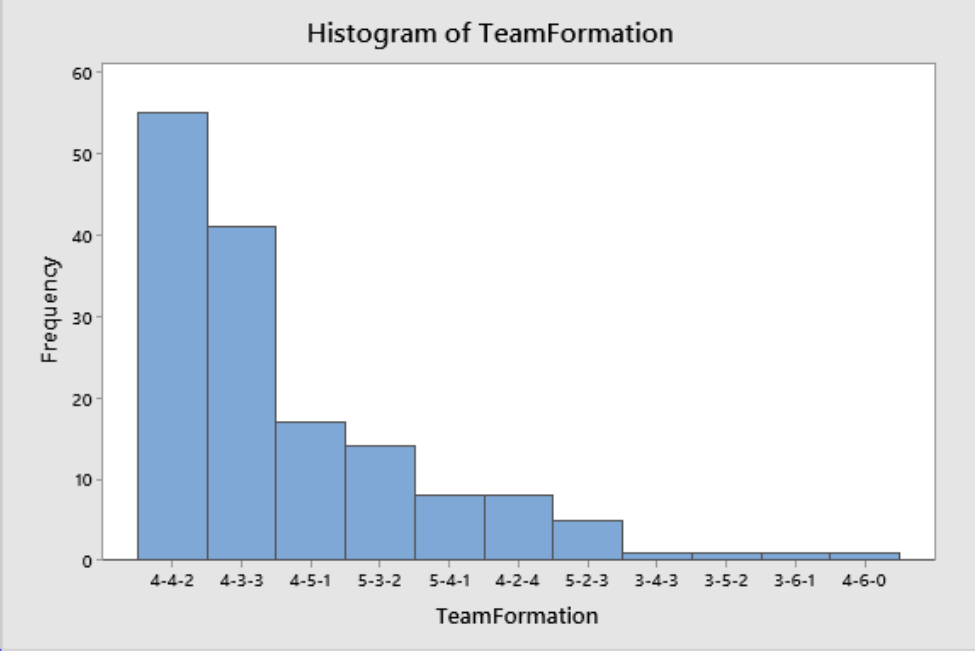
\includegraphics[scale=0.5]{images/Screen Shot 2020-02-17 at 8.29.29 PM.png}
\caption{Team Formation}
\end{center}
\end{figure}
\begin{figure}[ht]
\begin{center}
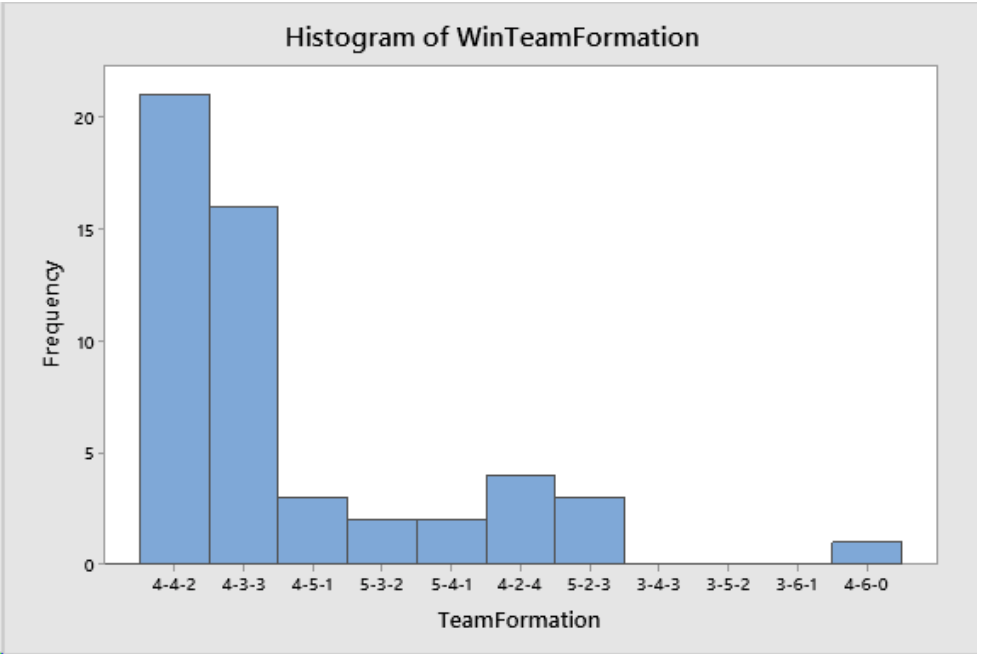
\includegraphics[scale=0.5]{images/Screen Shot 2020-02-17 at 8.29.34 PM.png}
\caption{Win Team Formation}
\end{center}
\end{figure}
%%%%%%%%%%%%%%%%%%%%%%%%%%%%%%
\end{document}
